
% JuliaCon proceedings template
\documentclass{juliacon}
\setcounter{page}{1}


%-------- user macros -----------------------------------------------------------
\usepackage{mathtools} %add-on and patches to amsmath  
\def\E{\mathbb{E}} 
%================================================================================

\begin{document}

% **************GENERATED FILE, DO NOT EDIT**************

\title{My JuliaCon proceeding}

\author[1]{Alberto Paoluzzi}
\affil[1]{Roma Tre University, Rome, Italy}

\keywords{Julia, Solid modeling, Geometric programming, Computational topology, Chain Complex, Cell Complex}



\maketitle

\begin{abstract}
Solid Modeling algorithms and applications usually demand very linked and pretty complex data structures, often denoted as ``non-manifold representations'' to remark the breadth of their domain. Conversely, we are implementing in Julia~\cite{bezanson2017julia} topological methods making only use of sparse binary or integer arrays, and their standard algebraic operations, like product, transposition and filtering, and standard topological operators of boundary and coboundary between linear spaces of chains generated by the cells of a space partition. 
We show computational methods to generate the 2D/3D space partition induced by a collection of 1D/2D/3D geometric objects. Methods and language are those of basic geometric and algebraic topology. Only sparse arrays are used to compute spaces and maps (the chain complex) from dimension zero to three.
In particular, we show how to build a space arrangement with general non-convex and non-contractible piecewise-linear cells, and how to compute Boolean operations between solid models generated by this approach, reducing them to standard tables of Boolean values.
\end{abstract}

%================================================================================
\section{Introduction}
%================================================================================

In this paper we discuss the current status of a novel approach to geometric computing, and its  implementation in Julia. Rather than using standard methods of geometric computing and solid modeling, normally built on top of complicated data structures, our work is mostly developed making advantage of    sparse arrays and their algebraic operations. In particular, this approach is established over basic concepts of algebraic topology, like cellular complexes, chain and cochain spaces and operators, and chain complexes.  Piecewise-linear algebraic topology allows to treat rather general complexes, with cells homeomorphic to polyhedra, \emph{i.e.},~to triangulable spaces, and hence possibly non convex and multiply connected. We use simplicial complexes, \emph{i.e.}, triangulations, just for graphics, where to stream triangles to the GPU is almost mandatory. 

At the knowledge of the author, there are no previous approaches to geometric and solid modeling that build over a similar framework, \emph{e.g}, to compute the \emph{chain complex} codifying the arrangement of $d$-space generated by a collection of ($d$-1)-geometric objects. A wide comparison with previous work in this field may be found in~\cite{TSAS:17,Dicarlo:2014:TNL:2543138.2543294}. 
After a short synthesis of basic algebraic topological 
concepts, this paper discusses the arrangement of space induced by solid objects, as the basis for resolution of solid-valued expressions. A survey of functions from our packages \texttt{LinearAlgebraicRepresentation}, \texttt{Triangle}, and \texttt{ViewerGL} follows. Simple examples generating pictures conclude the paper.

%================================================================================
\section{Linear Algebraic Representation}
%================================================================================

We summarize  in the following the concepts and definitions on which our \texttt{Lar} (Linear Algebraic Representation)~\cite{Dicarlo:2014:TNL:2543138.2543294} is based on. 

\subsection{Cell, Complex, Chain}
%--------------------------------------------------------------------------------
A $p$-cell $\sigma$ ($0\leq p\leq d$) is a piecewise-linear, connected, but possibly non-contractible $p$-manifold. An $r$-face $\tau$ of a $p$-cell $\sigma$ ($0\leq r\leq p$) is a $r$-cell contained in the frontier of $\sigma$.
A $d$-complex $\Lambda$ is a partition of a topological $d$-space $X$ in a discrete set of $p$-cells ($0\leq p\leq d$) such that: (a) $\sigma\in \Lambda$ implies $\tau\in \Lambda$ for all faces $\tau$ of $\sigma$; (b) the closure intersection of every pair of cells of $\Lambda$ is either in $\Lambda$ or the empty set. A $p$-chain can be defined as a subset of $p$-cells. To the $p$-chains can be given the structure of a (graded) linear space $C_p$ by defining (a) sums of chains with the same dimension, and (b) products times scalars in a field, with the usual properties. A basis $U_p$ for $C_p$ is the set of elementary chains $u_p$, given by single cells in $\Lambda_p$. Every chain $c\in C_p$ may be uniquely generated by a linear combination of the basis $U_p$. Once fixed the basis $U_p$, the coordinate representation of each $\sigma\in C_p$ is unique. This one is an ordered sequence of coefficients, either from $\{0,1\}$ (said unsigned rep.) or from $\{-1,0,+1\}$ (called signed representation).

\subsection{Boundary and coboundary operators}
%--------------------------------------------------------------------------------
Bondary operators are linear maps $\partial_p : C_p \to C_{p-1}$, ($1\leq p\leq d$). Coboundary operators are linear maps $\delta_p : C_p \to C_{p+1}$, ($0\leq p\leq d-1$). Once fixed the bases $U_{p-1}, U_{p}, U_{p+1}$, \emph{i.e.}, once fixed an ordering among the cells in each $\Lambda_p$, their matrix representations $[\partial_{p}]$ and $[\delta_{p}]$ are uniquely determined. 
It is worthwhile to remark the meaning of such matrices: once fixed the bases, the matrix $[M]$ of a linear operator $M: A\to B$ contains by columns the coordinate representation (\emph{i.e.}, the coefficients of the linear combination) of the $A$ basis expressed as linear combination of $B$ basis elements. This property is the conceptual key of our methods.

A \emph{$p$-cycle} is a chain \emph{without} boundary. It is a chain that the boundary operator $\partial_p$ sends to the kernel (zero-set) of $C_p$. In particular, the $j$-th column of $[\partial_p]$ contains a basis element $u_j\in U_p$ represented as a ($p-1$)-cycle, \emph{i.e.}, contains the coefficients of it as linear combination of elements of $U_{p-1}$. Such linear combinations are $(p-1)$-cycles, since $\partial_{p-1}\circ\partial_p = 0$.  In other words, the matrix $[\partial_2]$ represents the 2-cells in $\Lambda_2$ as 1-cycles (closed polygons) in $C_1$.  Analogously, $[\partial_3]$ contains by columns the 3-cells of $\Lambda_3$ as cycles (shells) made by 2-cells in $\Lambda_2$ (\emph{e.g.}, see Figure~\ref{fig:threecubes}d).

We  have already seen the topological equations $\partial_{p-1}\circ\partial_p = 0$ ($d\leq p\leq 2$) that guarantee the boundary of a boudary being empty. Think about the 2-disk $d \in C_2$ in the plane, with support $|d|\subset\E^2$. The circumference $c\in C_1$, with $|c| = |\partial_2\, d| \subset E^2$ is  a closed curve. In fact we have $\partial (\partial\, c) = 0$. In our case, where cells live in Euclidean spaces, chain spaces $C_p$ can be identified with their dual spaces of $p$-cochains $C^p$, that are spaces of maps $\mu^p: C_p\to \mathbb{F}$ from $p$-chains to the field $\mathbb{F}$ of coefficients. In this case we have $C^p = C_p^\top$, and hence $[C^p] = [C_p]^t$. The matrix-vector multiplication $[\partial_p][c]$ provides the (coordinate representation of) the ($p$-1)-cycle on the frontier of $c$, whereas $[\delta^p][c]$ gives the (coordinate repre. of) the ($p$+1)-chain made by all ($p$+1)-cells incident on $c$.

\begin{figure}[htbp] %  figure placement: here, top, bottom, or page
   \centering
   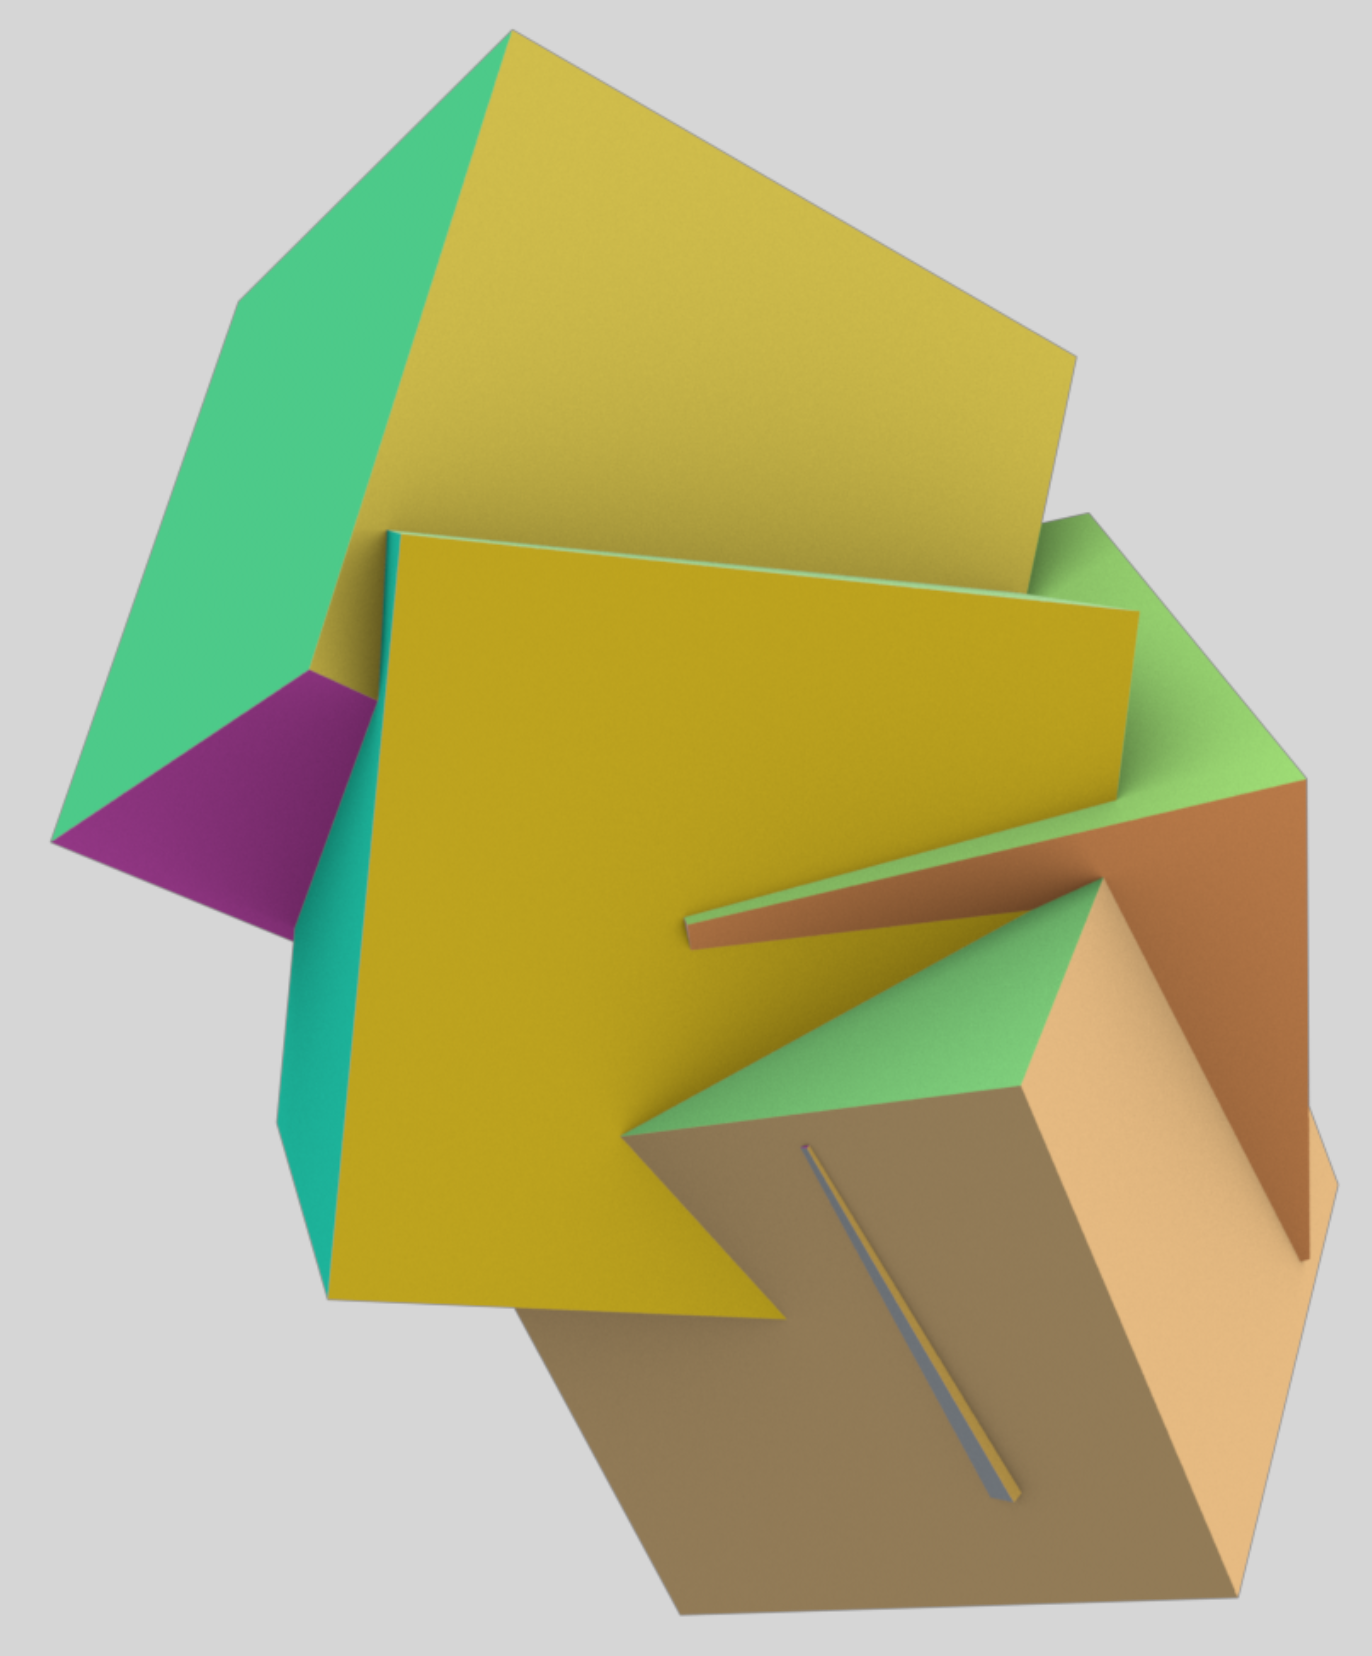
\includegraphics[width=0.4\linewidth]{figs/image1.png}%
   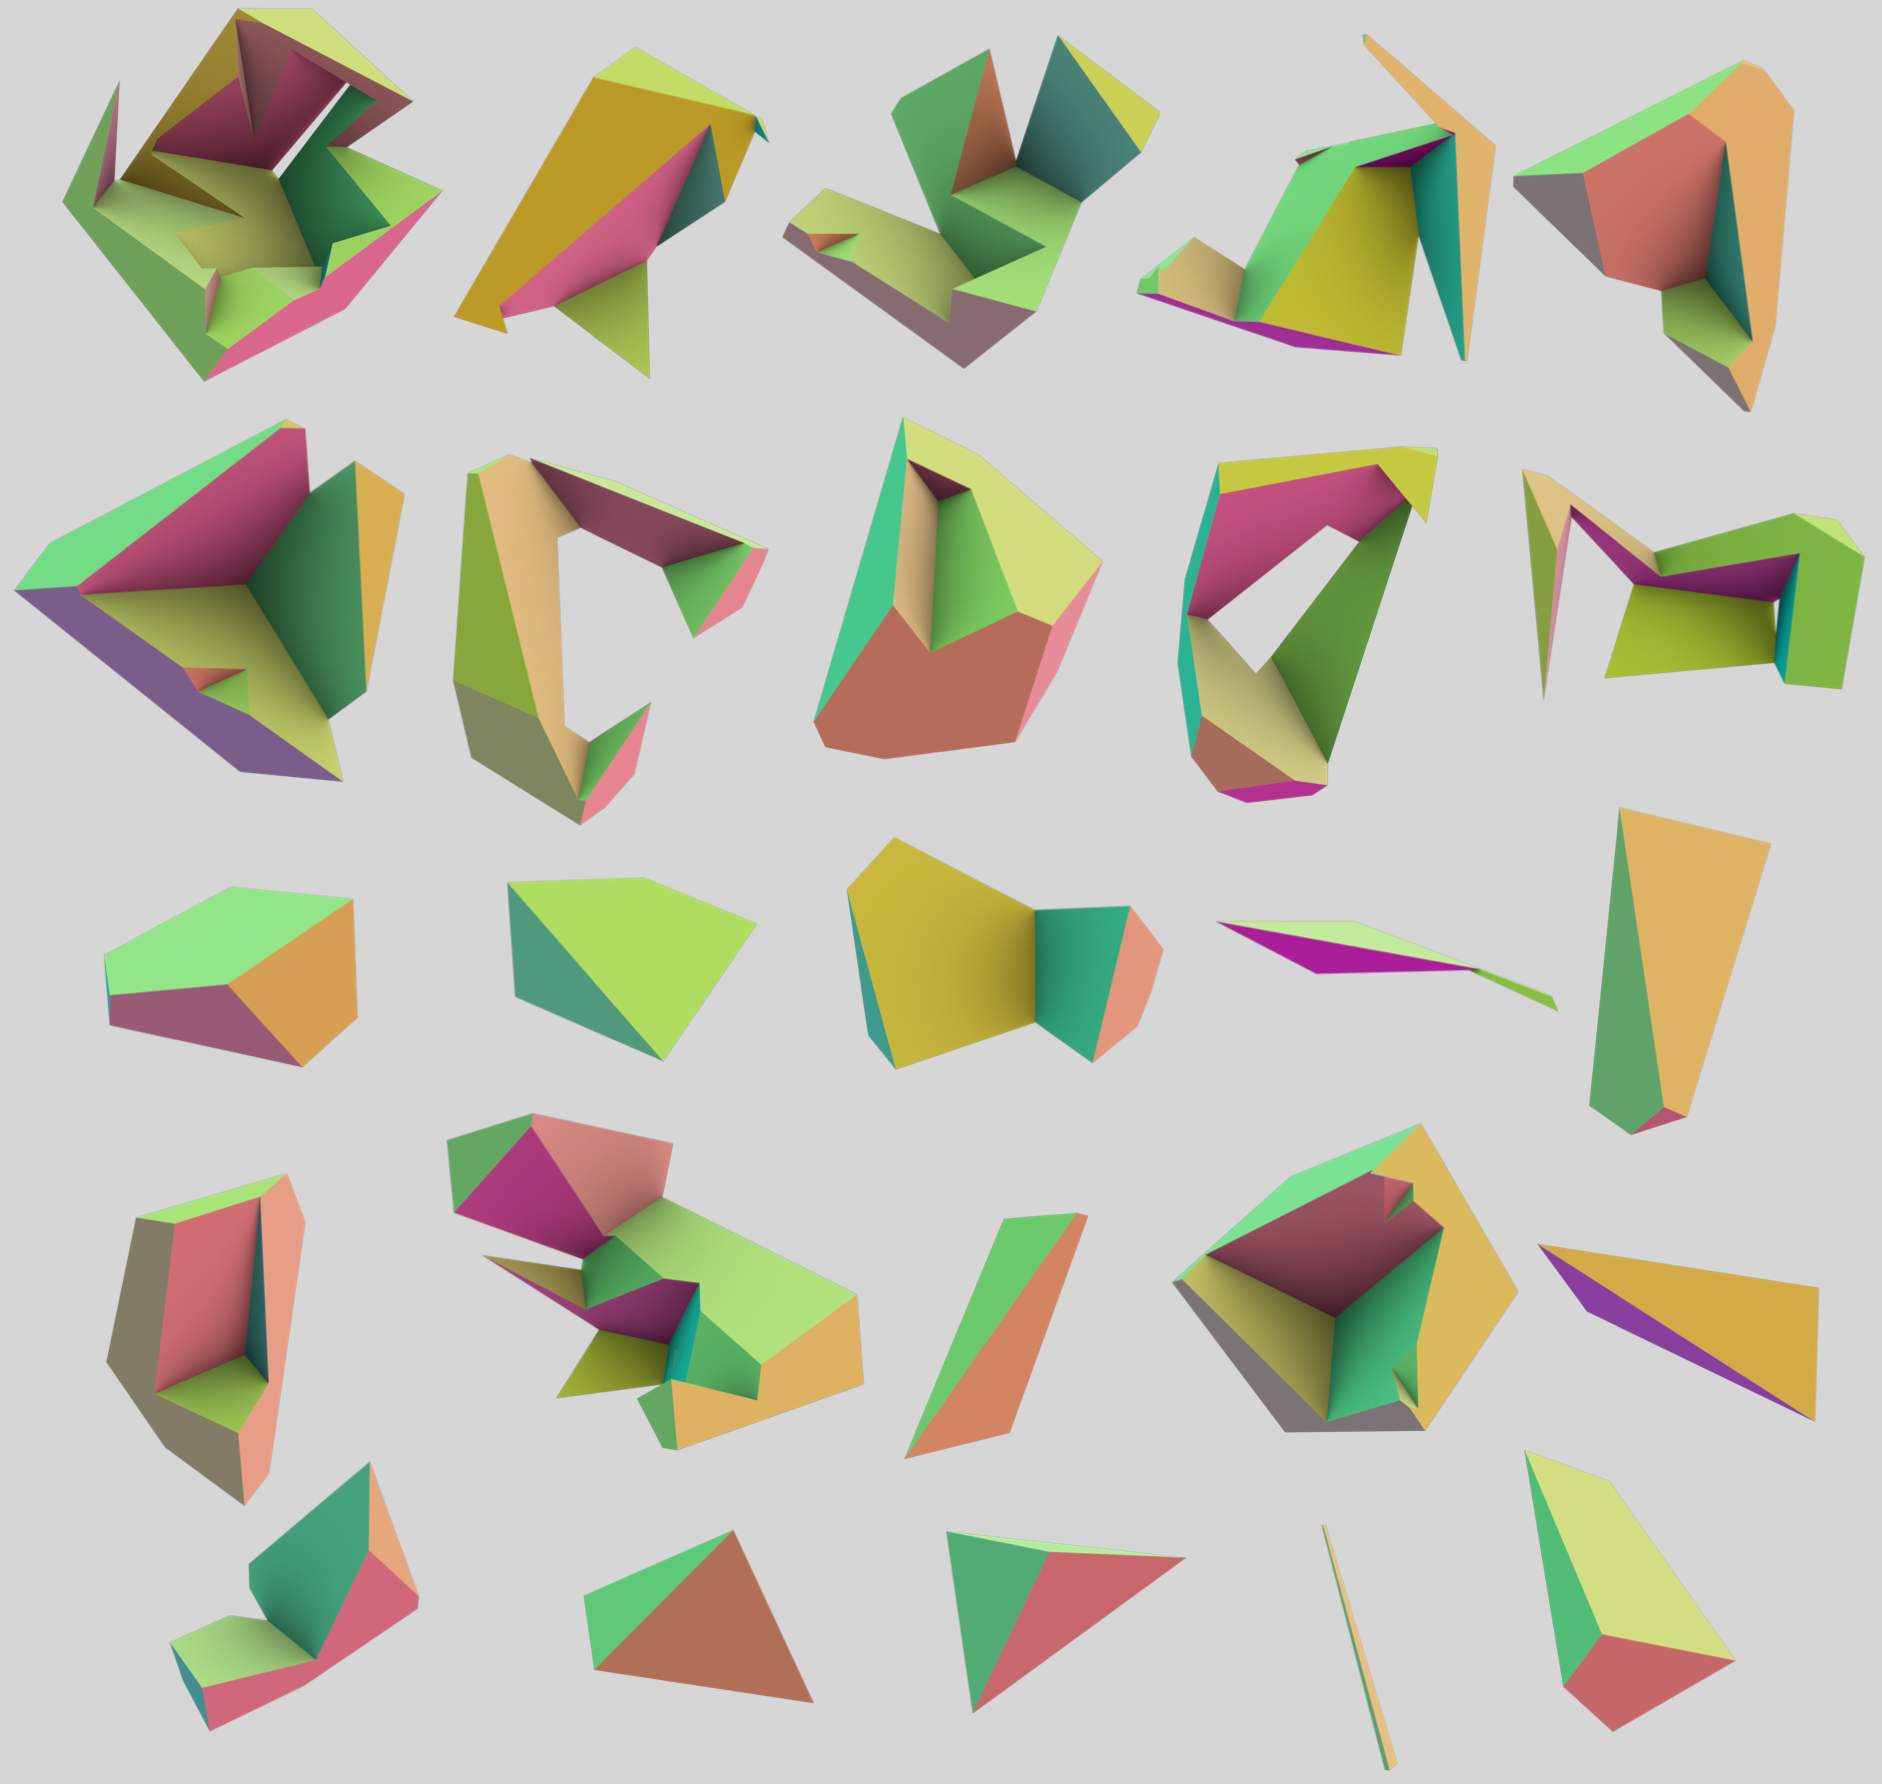
\includegraphics[width=0.6\linewidth]{figs/image2.png}%
   \caption{The 3-cells of the arrangement of $\E^3$ generated by a collection of five random cubes.
   The 3-cells are here not in scale, and suitably rotated to better show their complex structure.
   Their assembly provides the union of the five cubes.
   Each \emph{3-cell is given} by \emph{a column} of the \emph{sparse matrix} of \emph{chain map} $\partial_3: C_3\to C_2$,  with values in $\{-1,0,1\}$.}
   \label{fig:example}
\end{figure}



\subsection{Incidence/adjacency operators}
%--------------------------------------------------------------------------------
Specialized data structures are commonly used to efficiently answer the queries about the incidence and adjacecy relations between boundary elements (vertices, edges and faces), in order to implement the various geometric and topological algorithms of solid modeling. Given the three sets \texttt{V}, \texttt{E}, and \texttt{F} (vertices, edges and faces), ${3\times 3}$ binary relations \texttt{VV}, \texttt{VE}, \texttt{VF}, \texttt{EV}, \texttt{EE}, \texttt{EF}, \texttt{FV}, \texttt{FE}, \texttt{FF} are used. Several different combinations of such relations have been defined as specialized data structures, with the aim of minimizing the time and space complexity of algorithms on solid models.

It is easy to see that each relation can be computed by a proper combination of one or two (co)boundary matrices, possibly transposed. Their ordered list follow: $\texttt{VV}\equiv[\partial_1][\delta_0]$, $\texttt{VE}\equiv[\partial_1]$, $\texttt{VF}\equiv[M_2]^t$, $\texttt{EV}\equiv[\partial_1]^t$, $\texttt{EE}\equiv[\delta_0][\partial_1]$, $\texttt{EF}\equiv[\partial_2]$, $\texttt{FV}\equiv[M_2]$, $\texttt{FE}\equiv[\delta_1]$, $\texttt{FF}\equiv[\delta_1][\partial_2]$, where $M_p$ is the sparse binary \emph{characteristic matrix} of $p$-cells, that holds by rows the images of characteristic functions of $p$-cells as subsets of $0$-cells (vertices).

A typical topological query may be asked as: ``what edges (elementary 1-chains) are adjacent to edge $e$?''
The \texttt{Lar} answer is computed as the product $[\delta_0][\partial_1][e]$, where $[e]$ is the coordinate representation of $e\in C_1$ (a sparse column vector with just one non-zero element) and, of course, the matrix $[\delta_0][\partial_1] =: [\texttt{EE}]$ was computed in advance, and once for all.

The cardinality of such incidence/adjacency algebraic tools between p-cells and q-cells $(0\leq p,q \leq 2)$ is equivalent to that of relations itself~\cite{Woo:85}, in force of their sparsity.  For example, $\#\texttt{EV} = O(Space([\delta_1]) = 2\#\texttt{E}$), where \texttt{V} are the vertices of a solid B-rep and \texttt{EV} are binary incidences of edges with vertices. Every set of local queries about the $3\times 3$ incidences/adjacencies between cells can be answered by multiplication, via software kernels for \emph{sparse matrix} product and transposition, just by collecting the coordinate vectors of unit chains, ``subject''  of elementary queries, as \emph{columns} of a sparse $Q$ matrix, and by left-multiplying $Q$ times one/two operator matrices $[\partial_1]$ and/or $[\partial_2]$, suitably ordered and/or transposed~\cite{Dicarlo:2014:TNL:2543138.2543294}, to get the algebraic equivalent of multiple database queries at once.

%================================================================================
\section{Arrangement Algorithms}
%================================================================================

A \emph{chain complex} is a short exact sequence of graded linear spaces \(C_p\) of (co)chains, with linear
boundary/coboundary maps \(\partial_p\) and
\(\delta_p=\partial_{p+1}^\top\): 
\[ 
C_\bullet = (C_p, \partial_p) := 
C_3 \ 
\substack{
\delta_2 \\
\longleftarrow \\[-1mm]
\longrightarrow \\
\partial_3 
}
\ C_2 \ 
\substack{
\delta_1 \\
\longleftarrow \\[-1mm]
\longrightarrow \\
\partial_2 
}
\ C_1 \ 
\substack{
\delta_0 \\
\longleftarrow \\[-1mm]
\longrightarrow \\
\partial_1 
}
\ C_0 .
\] 

The subject of Reference~\cite{TSAS:17} is the computation of the chain complex $C_\bullet = (C_p,\partial_p)$, starting from some representation\footnote{Our prototype implementation in\\ \href{https://github.com/cvdlab/LinearAlgebraicRepresentation.jl}{\scriptsize \texttt{https://github.com/cvdlab/LinearAlgebraicRepresentation.jl}}, makes use of the \texttt{Lar} representation~\cite{Dicarlo:2014:TNL:2543138.2543294}, on which this approach strongly relies.} of an input set $\mathcal{S}$ of ($d$-1)-complexes. In particular, we compute the matrices of the linear maps $\partial_p$ (and their duals $\delta_{p-1}$)  between chain spaces $C_p$. All definitions and more examples are given in Reference~\cite{TSAS:17}. We describe here the main steps of space decomposition in reverse order, starting from the last operation, because of possible iteration on dimensions, starting from 3D.


\subsection{Topological gift wrapping}
%--------------------------------------------------------------------------------
The main goal is to compute, starting from ($d$-1)-dimensional geometric object, the $d$-cells of the space partition (arrangement) generated by them. Examples of input include, but are not limited to: line segments, quads, triangles, polygons, meshes, pixels, voxels, volume images, B-reps, \emph{etc.} 
In mathematical terms, a geometric object is a topological space embedded in some $\E^d$ .

The topological method introduced in~\cite{TSAS:17} is reminiscent of the ``gift-wrapping'' algorithm~\cite{Cormen:2009:IAT:1614191,Jarvis:1973:ICH} for computing convex hulls of 2D and 3D discrete sets of points, but it works with higer-dimensional cells instead with points, and is mostly based on applications of boundary and coboundary operators. Our \texttt{TGW} (Topological Gift Wrapping) algorithm~\cite{TSAS:17} takes a sparse matrix $[\partial_{d-1}]$ as input and produces in output the \emph{unknown} sparse matrix  $[\partial_{d}^+]$, augmented with the outer cell. A geometric embedding function $\mu: X_0\to\E^d$ is used to compute the angular ordering, around some ($d$-2)-cells, of ($d$-1)-basis elements in the boundary's coboundary, while wrapping up a ($d$-1)-cycle, as illustrated in Figure~\ref{fig:3D}. The built cycles are set up as columns of $[\partial_d]$, in the construction of a $C_d$ basis.


\begin{figure*}[htbp] %  figure placement: here, top, bottom, or page
\hfill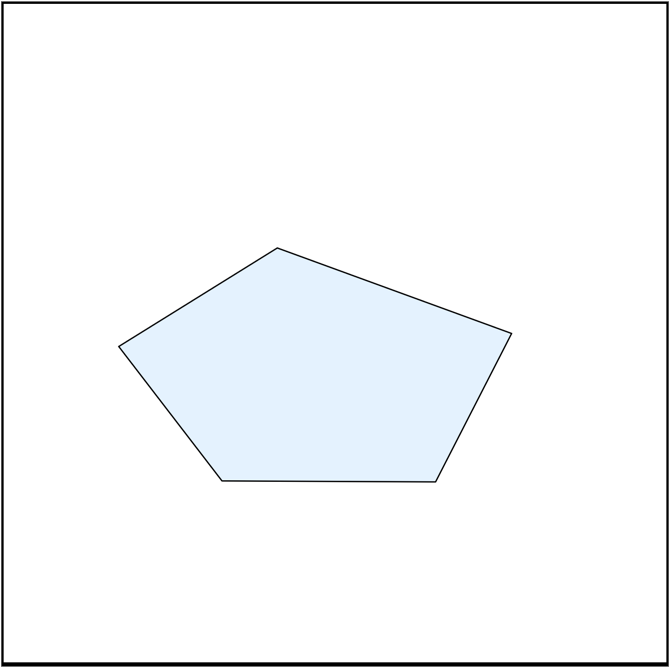
\includegraphics[height=0.15\textwidth,width=0.1428\textwidth]{figs/3D1a.png}%
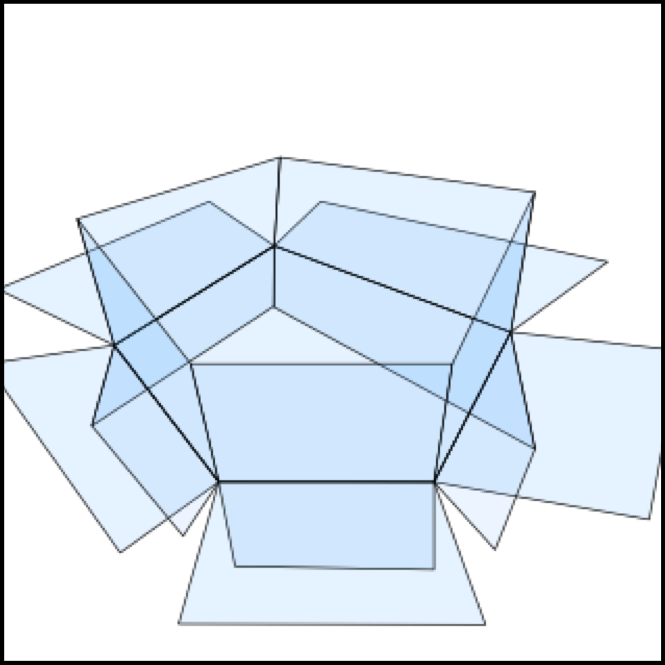
\includegraphics[height=0.15\textwidth,width=0.1428\textwidth]{figs/3D2.png}%
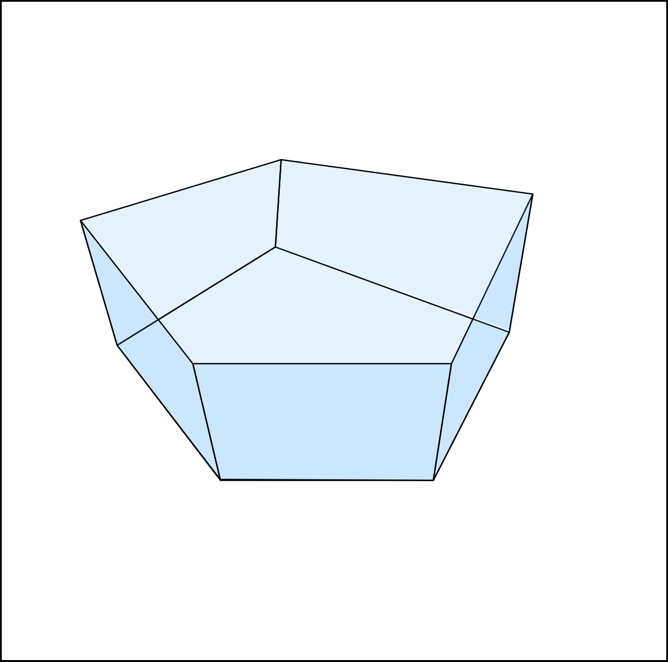
\includegraphics[height=0.15\textwidth,width=0.1428\textwidth]{figs/3D3b.png}%
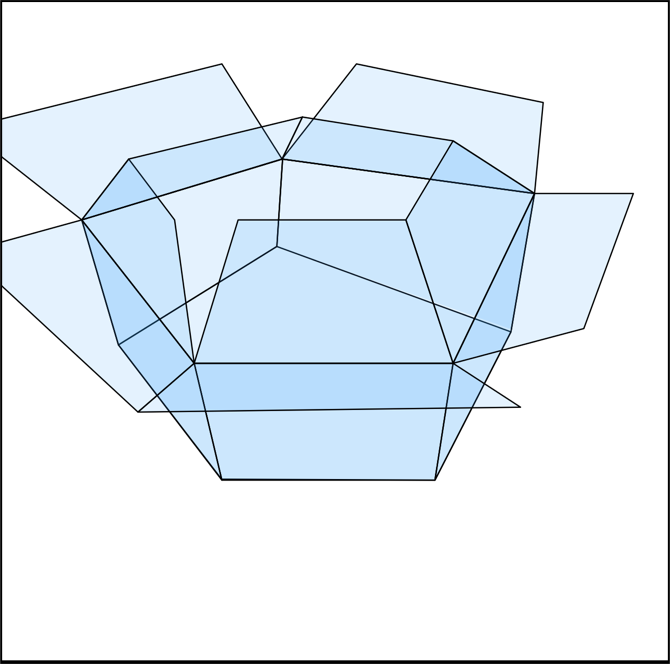
\includegraphics[height=0.15\textwidth,width=0.1428\textwidth]{figs/3D4a.png}%
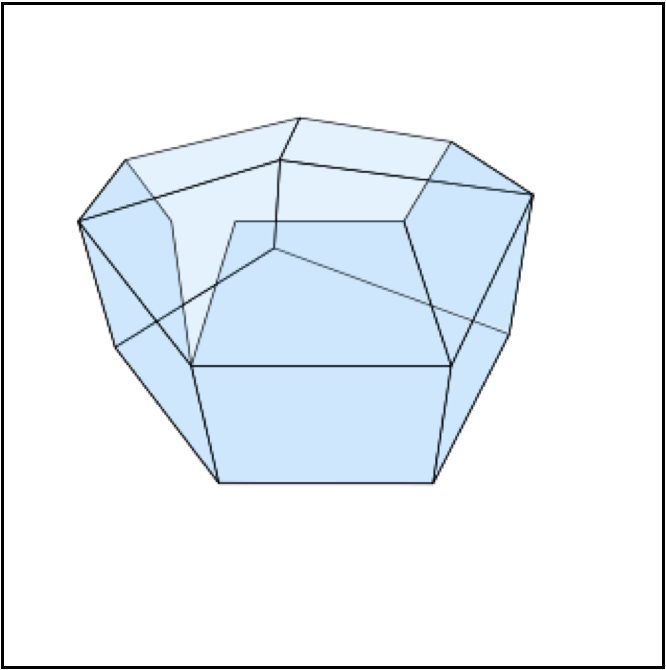
\includegraphics[height=0.15\textwidth,width=0.1428\textwidth]{figs/3D5a.png}%
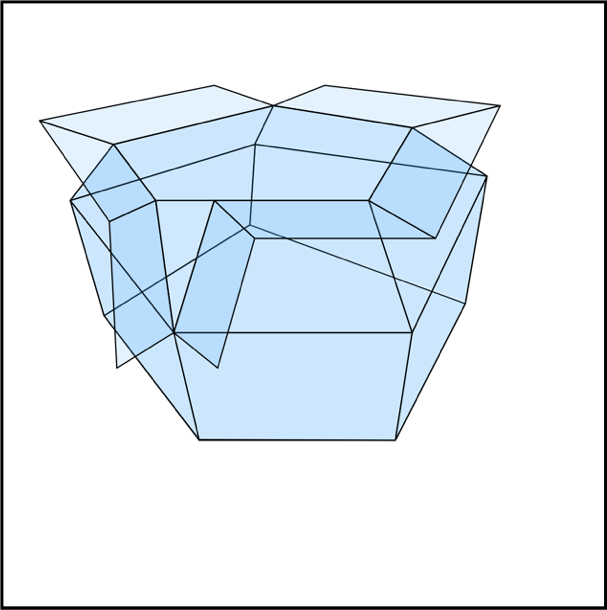
\includegraphics[height=0.15\textwidth,width=0.1428\textwidth]{figs/3D6b.png}%
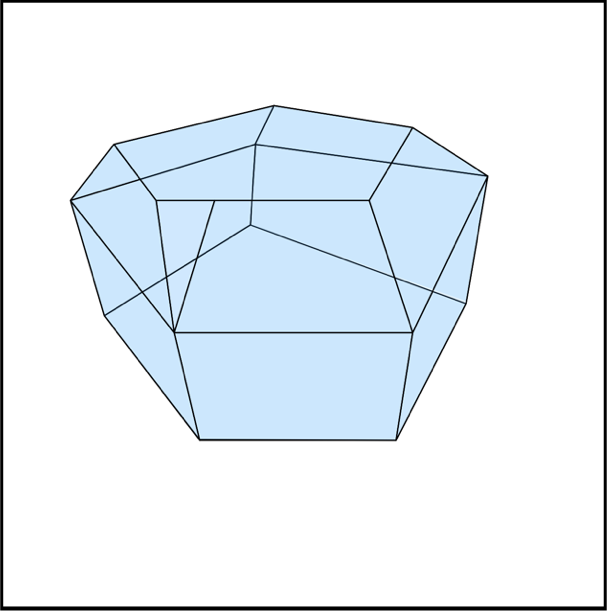
\includegraphics[height=0.15\textwidth,width=0.1428\textwidth]{figs/3D7a.png}

{\footnotesize\hspace{.06\textwidth}(a)\hfill(b)\hfill(c)\hfill(d)\hfill(e)\hfill(f)\hfill(g)\hspace{.06\textwidth}}

\caption{Extraction of a minimal 2-cycle from $\mathcal{A}(X_2)$: (a) initial (0-th) value for $c\in C_2$; (b) cyclic subgroups on  $\delta\partial c$; (c)~1-st value of $c$; (d) cyclic subgroups on $\delta\partial c$; (e) 2-nd value of $c$; (f) cyclic subgroups on $\delta\partial c$; (g) 3-rd value of $c$, such that $\partial c=0$, hence stop.}
   \label{fig:3D}
\end{figure*}


\subsection{Merge of 2-skeletons}
%--------------------------------------------------------------------------------
The input to the computational pipeline is a collection $\mathcal{S}$ of geometric objects that do not necessarily constitute a cellular complex, since they can intersect out of cell boundaries. The first step is hence the computation of mutual interctions of their 2-skeletons, \emph{i.e.}, of their sets of 2-cells (for a 3D problem), or their 1-skeletons (for a 2D problem). This phase is executed by intersecting independently each 2-cell $\sigma\in\mathcal{S}_2$ with all 2-cells which might intersect it. Their subset is denoted $\mathcal{I}(\sigma)$ and is computed using efficient spatial indices on the containment boxes of 2-cells. In particular, each $\mathcal{I}(\sigma)$ is given by the intersection of outputs of $d$ independent queries over one-dimensional interval-trees built upon the input.

It may be interesting to remark that the \texttt{merge} algorithm is embarrassingly parallel, and is implemented in Julia making use of two \texttt{Channel}s to ditribute the jobs to workers and to return the output to the master node. This more efficient strategy is quite unusual in Solid Modeling, where even recent variadic approaches~\cite{Zhou:2016:MAS:2897824.2925901} iteratively intersect a new operand against the cell complex generated by the previous operations. 


\begin{figure}[htbp] %  figure placement: here, top, bottom, or page
   \centering
   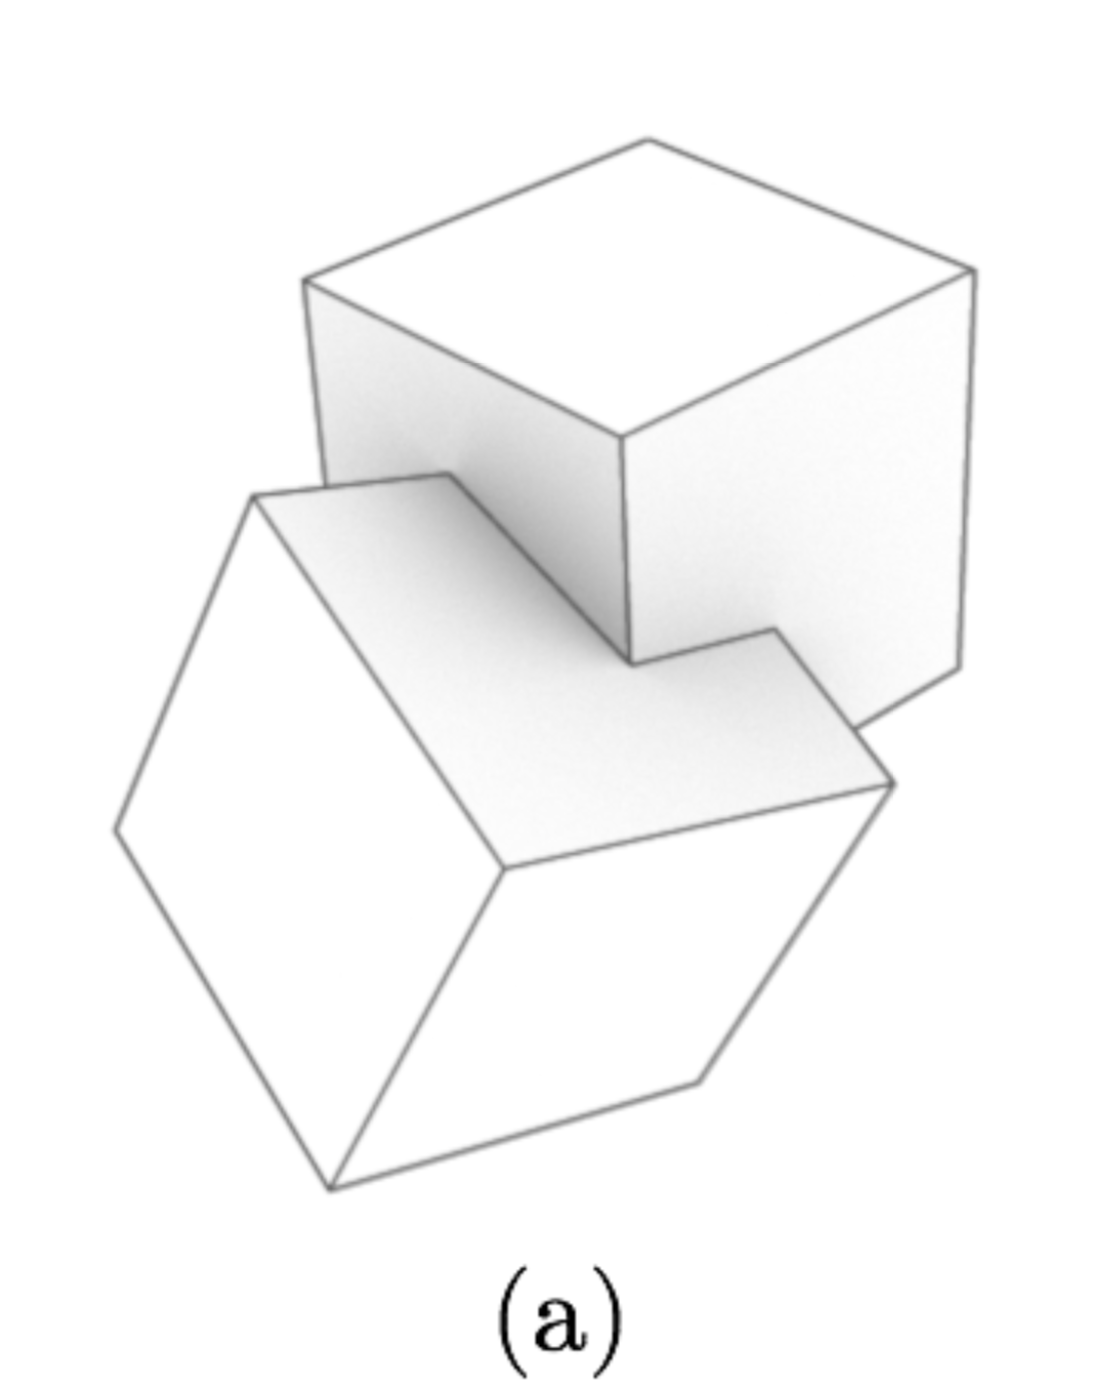
\includegraphics[width=0.25\linewidth]{figs/1.png}%
   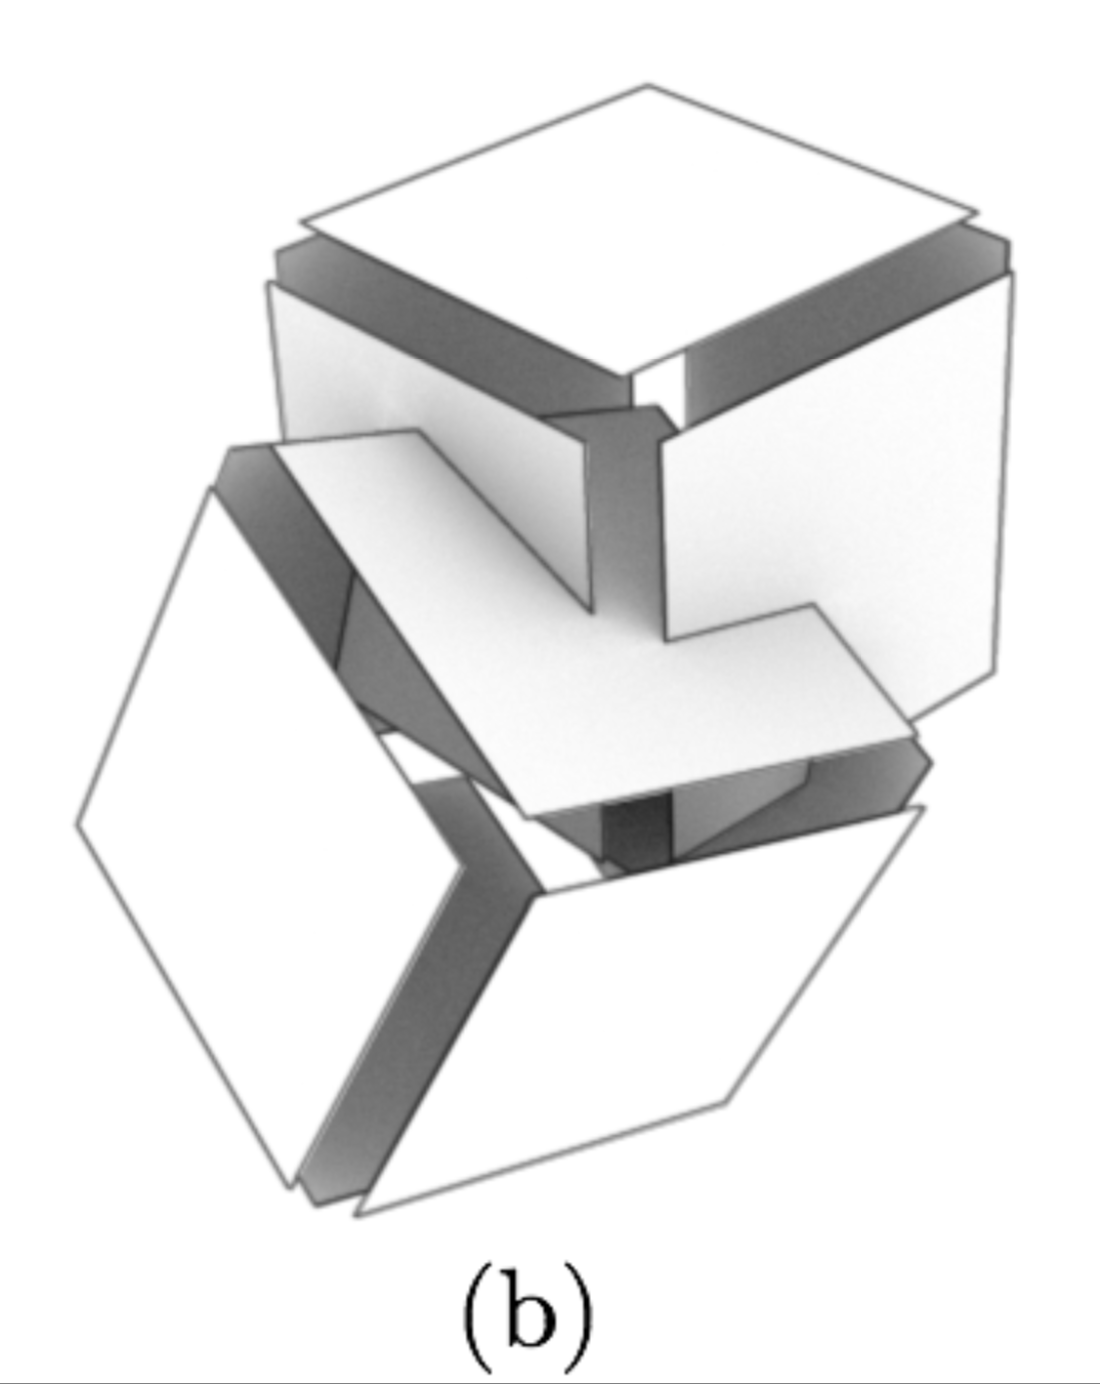
\includegraphics[width=0.25\linewidth]{figs/2.png}%
   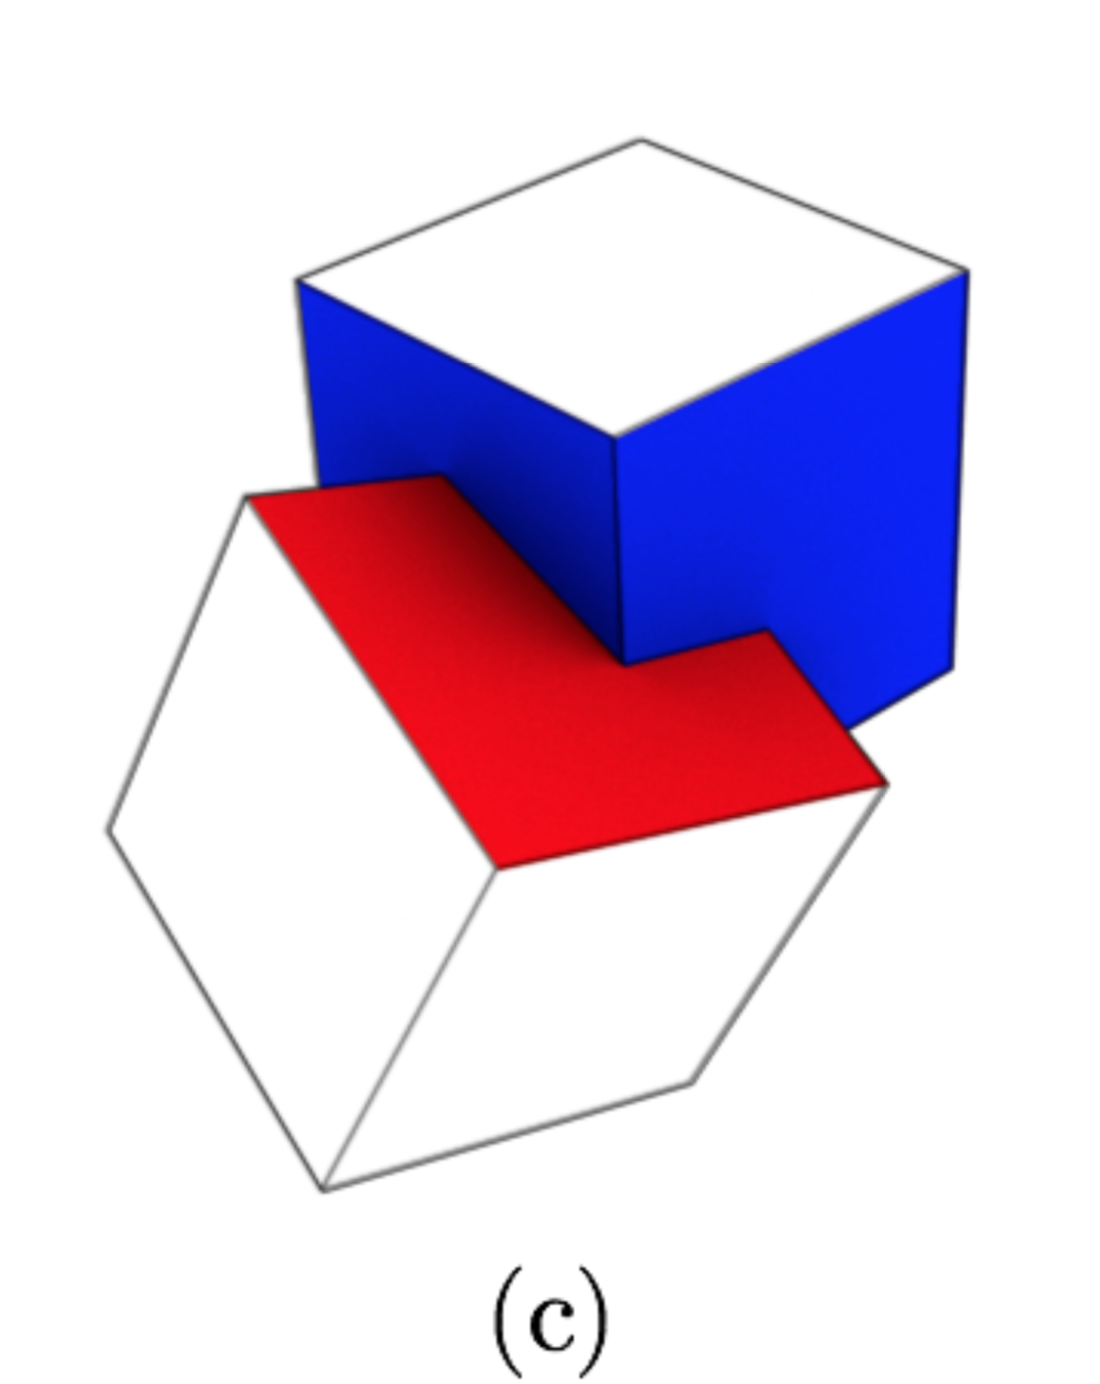
\includegraphics[width=0.25\linewidth]{figs/3.png}%
   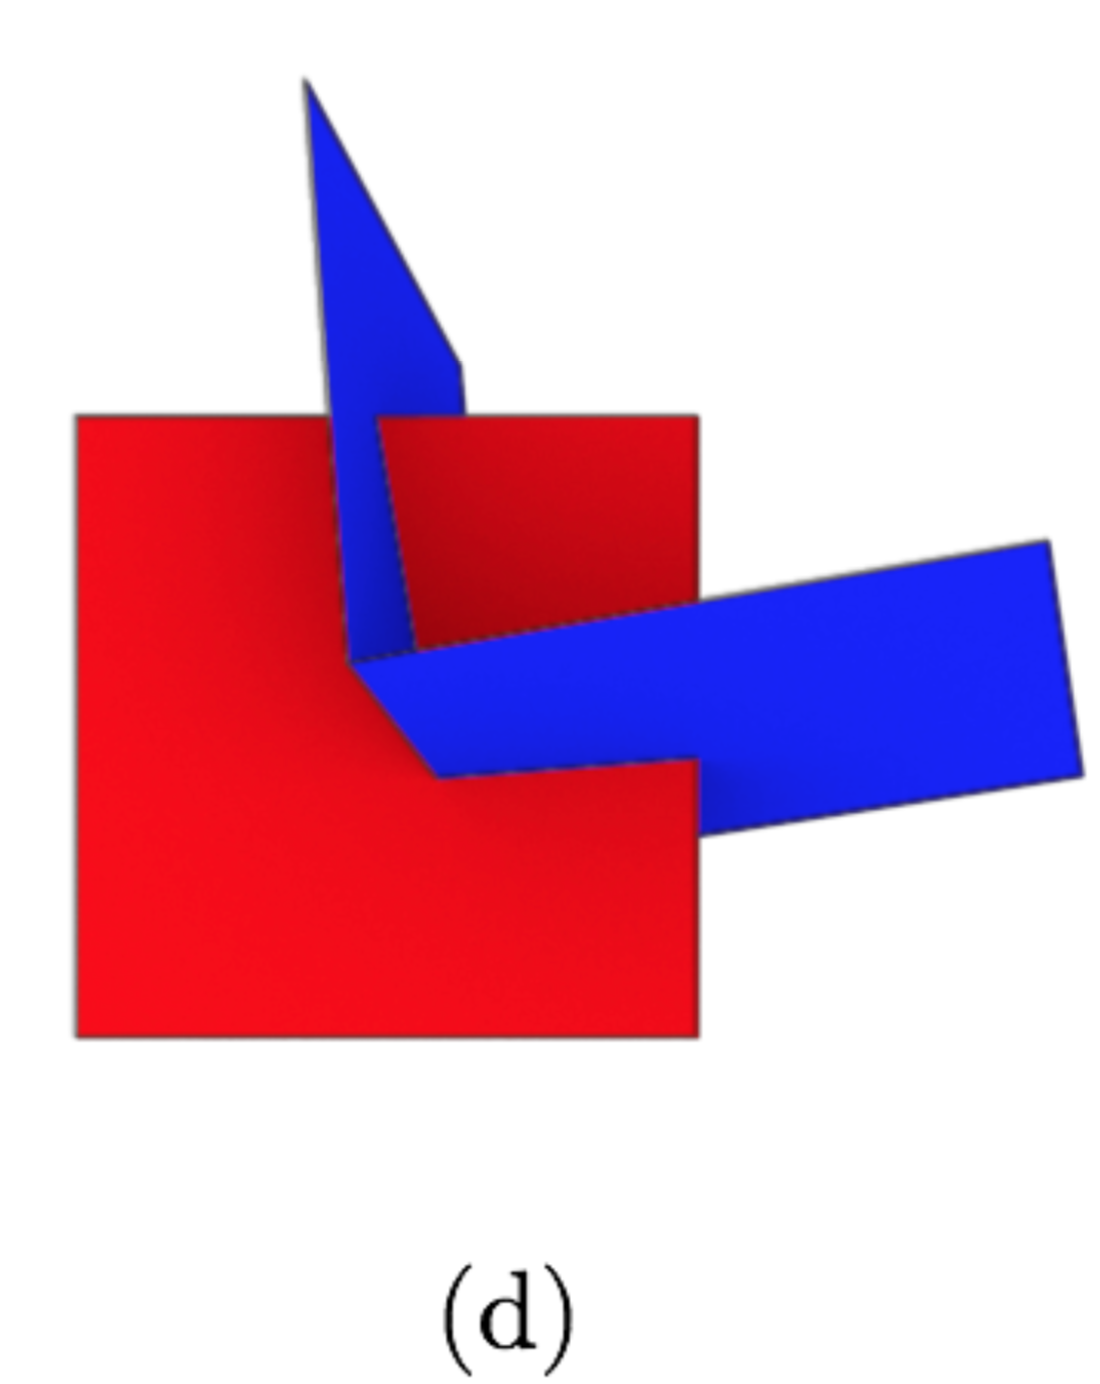
\includegraphics[width=0.25\linewidth]{figs/4.png} 

   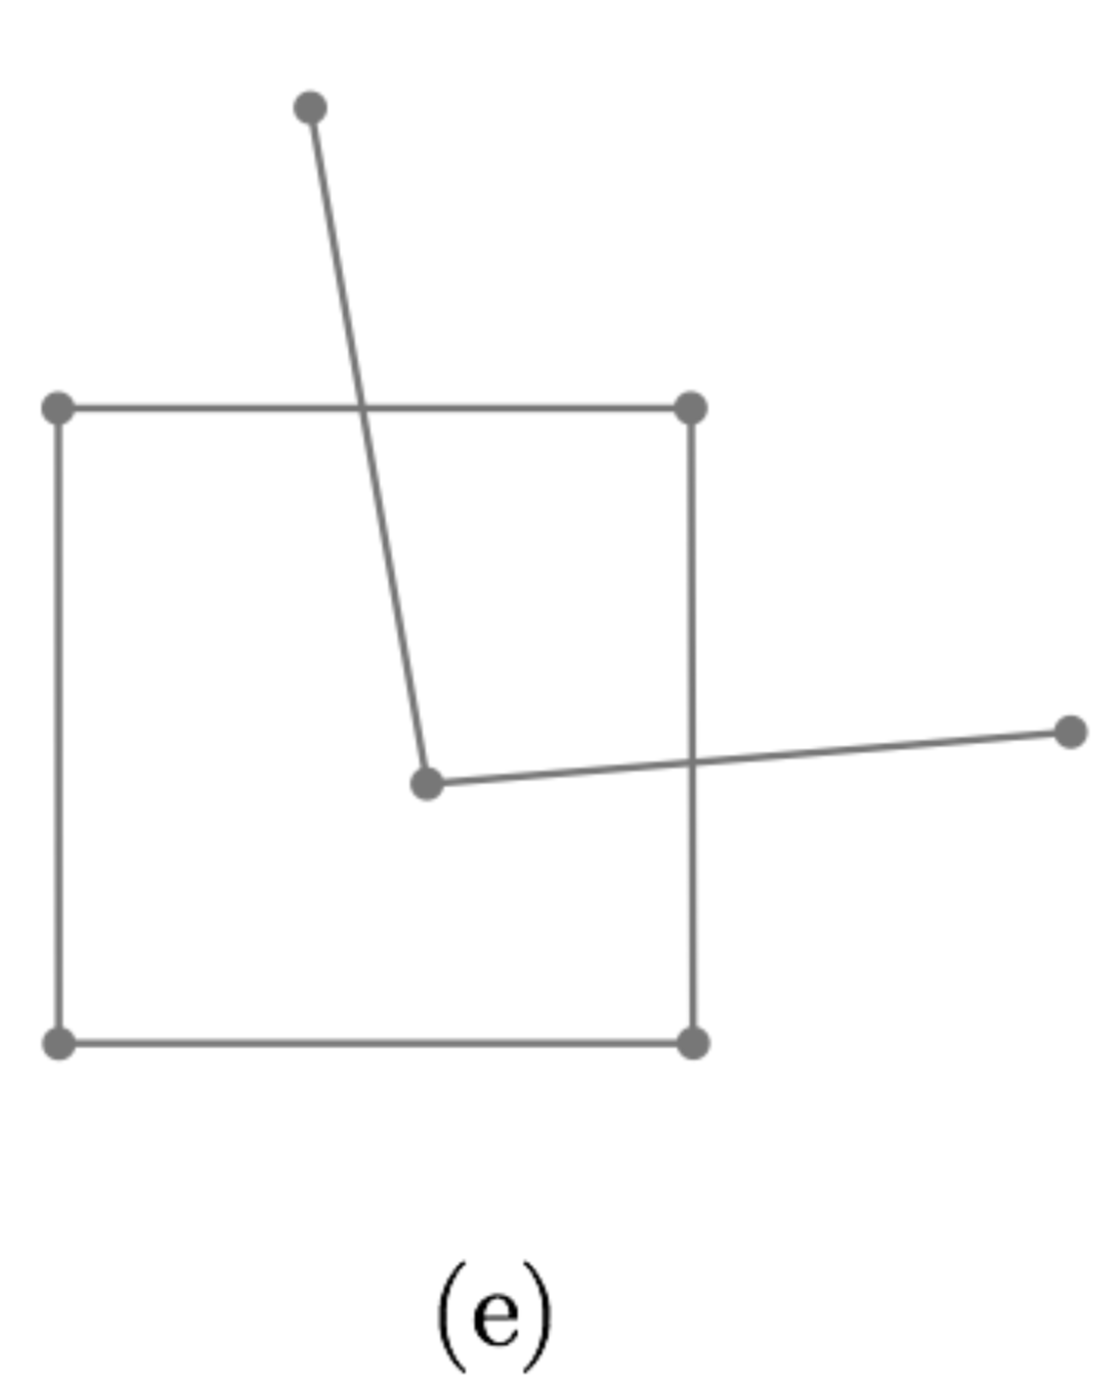
\includegraphics[width=0.25\linewidth]{figs/5.png}%
   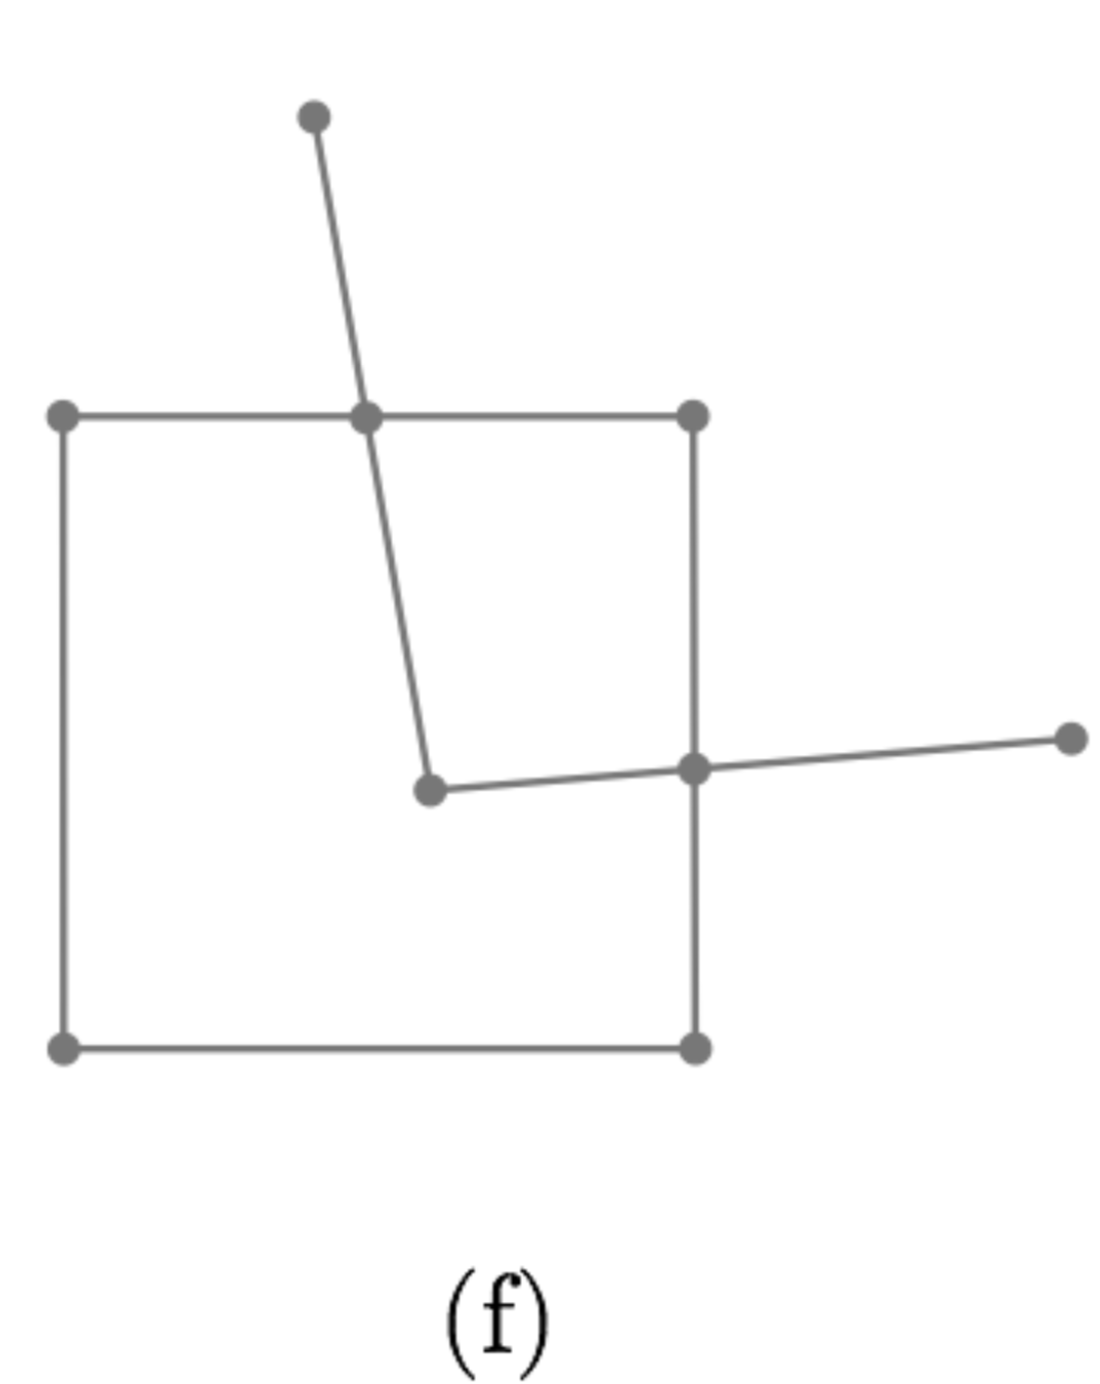
\includegraphics[width=0.25\linewidth]{figs/6.png}%
   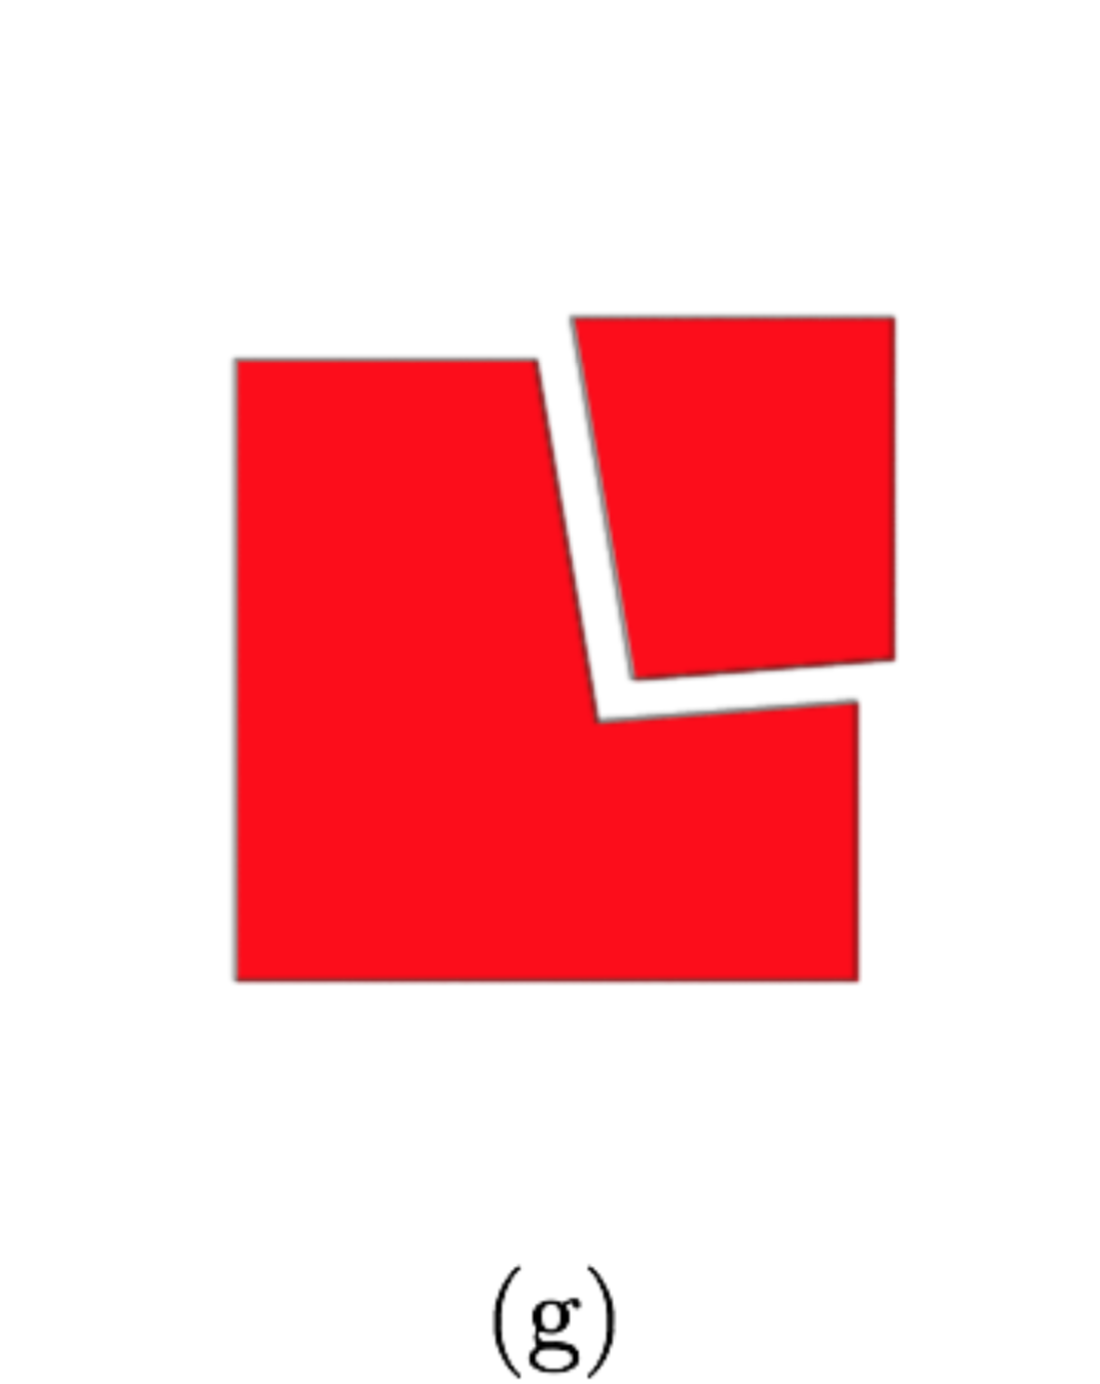
\includegraphics[width=0.25\linewidth]{figs/7.png}%
   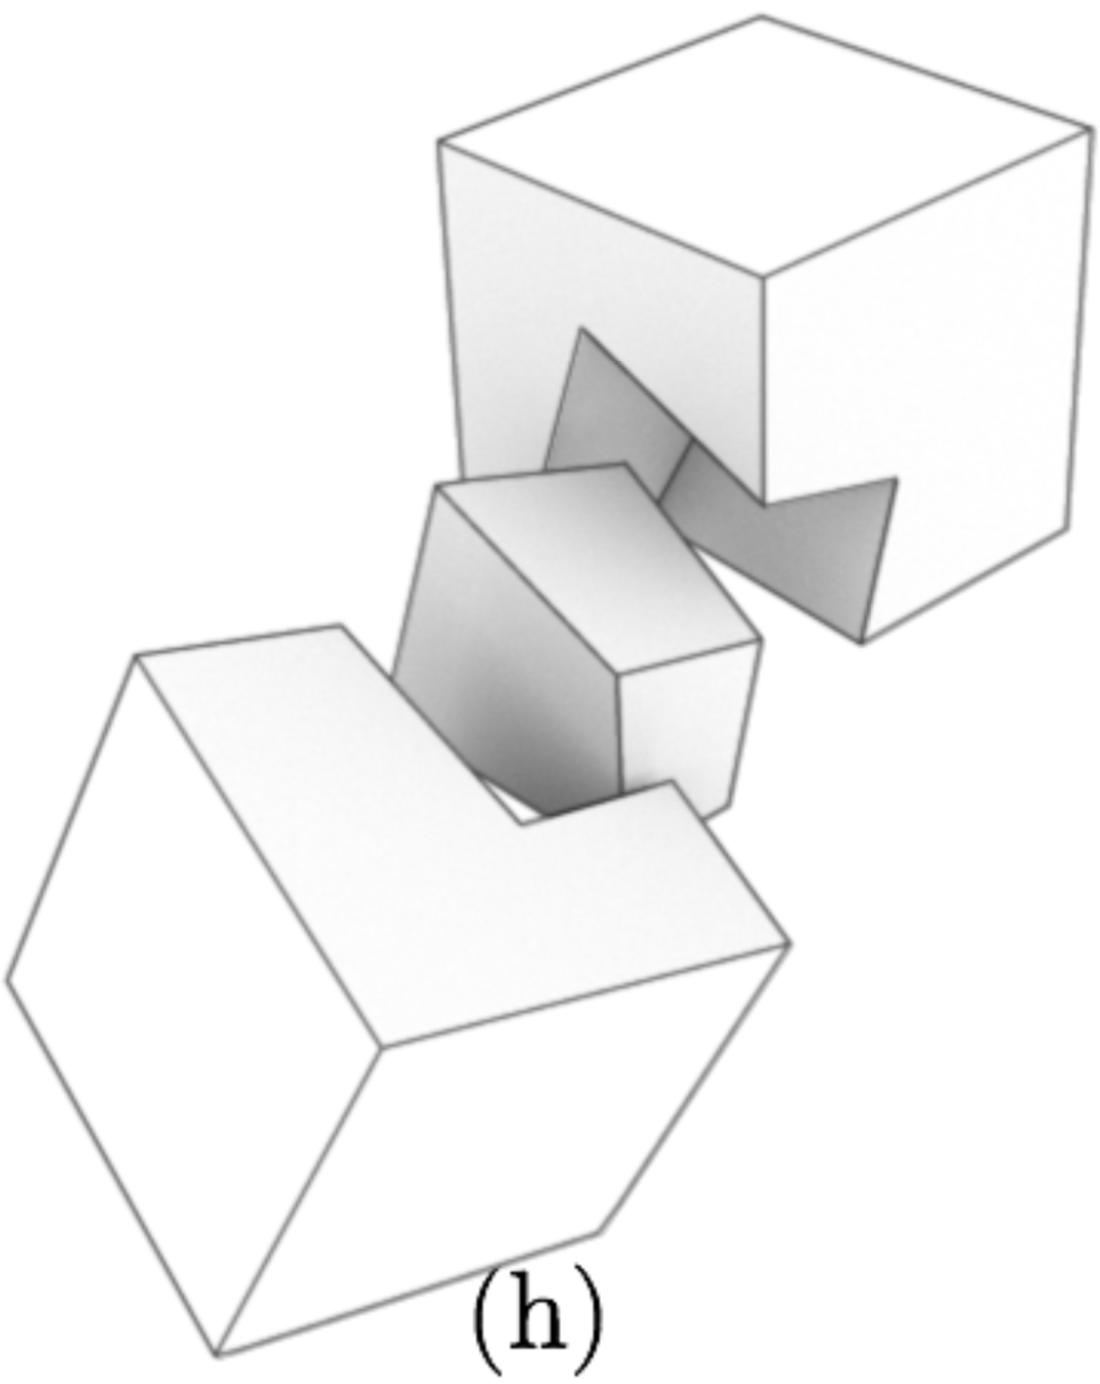
\includegraphics[width=0.25\linewidth]{figs/8.png}%
   
   \caption{Cartoon display of the computational pipeline: (a) two solids in $\mathcal{S}$; (b) the exploded input collection $\mathcal{S}_2$ in $\E^3$; (c) 2-cell $\sigma$ (red) and the set $\Sigma(\sigma)$ (blue) of possible intersection; (d)  $\sigma\cup\Sigma$ affinely mapped on $z=0$; 
   (e)~reduction to a set of 1D segments in $\E^2$ via intersection with $z=0$; (f) pairwise intersections; (g) exploded $U_2$ basis of $C_2$ generated as columns of $\partial_2: C_2 \to C_1$; (h) exploded $U_3$ basis of $C_3$ generated as columns of operator's $\partial_3: C_3 \to C_2$ sparse matrix, via the \texttt{TGW} algorithm in 3D.    }
   \label{fig:process}
\end{figure}


The independent processing of 2-cells is made possible by considering and enforcing the congruence (i.e.~the boundary compatibility) between adjacent fragmented cells. Hence, each input 2-cell $\sigma$ is fragmented in 2D independently from each other.  For this purpose,  a suitable affine transformation maps each set $\{\sigma\}\cup\mathcal{I}(\sigma)$ and puts $\sigma$ into the $z=0$ subspace.


\subsection{Reduction to line intersection in 2D}
%--------------------------------------------------------------------------------
At this point the single 3D arrangement problem is reduced to a collection of several independent 2D arrangement problems, one-to-one with the 2-cells in the 3D input. Every 2-cell in $\mathcal{I}(\sigma)$ is independently intersected (in parallel) with $z=0$, so providing a number $n$ of line segment sets $\mathcal{S}_1$ for independent computation of the 2D arrangement generated by it. The computational pipeline is depicted as cartoon in Figure~\ref{fig:process}. In particular: each set of line segments is mutually intersected (using again two 1D interval-trees of containment boxes of segments for acceleration); the dangling edges and subgraphs are removed from the generated linear graph; and the \texttt{TGW} is used in 2D to build the matrix $[\partial_2]$ of the arrangement, and the corresponding basis of elementary 2-chains (2-cells) of the  $\sigma$ cell decomposition.


\subsection{Congruence of 2D arrangements}
%--------------------------------------------------------------------------------
Each 2-complex $X_\sigma$ providing an independent arrangement of 2-space, is transformed back in 3D using the inverse affine transformation of $\sigma$. Here, congruent cells (e.g., edges member of the boundary of two or more fragmented faces) must be identified as belonging to the same equivalence class, and substituted by a single instance, so implementing a set quotient operation on fragmented cells. Numerical identification of vertices via dictionaries having arrays of floats as keys (permitted by Julia) are used for this purpose. Once identified congruent vertices, the identification of congruent edges and faces is done using their canonical \texttt{Lar} representation, \emph{i.e.,} the ordered arrays of integer indices of vertices. 

%================================================================================
\section{Variadic Boolean Operations}
%================================================================================

When the unknown sparse boundary matrix $[\partial_3]$ has been generated by \texttt{TGW} in 3D, the computation of any Boolean operation or solid-valued expression, including solid arguments and Boolean operators, is actually straightforward\footnote{Even if not yet implemented.}. Let us note that the arrangement itself corresponds to the output of a union operation.
To compute any general solid-valued expression, it suffices to suitably store the dependencies, of each possibly fragmented 2-cell of resulting 3-cells, from the input 2-cells that generated it, i.e. from its ``father(s)". This storing allows to reconstruct the containment relations of arrangement's 3-cells with their parents, and hence to write truth tables having them on columns, and the original solids (or their boundaries) on the rows.
It is worthwhile to note that most of the required information is already coded by the non-zero coefficients of $[\partial_3]$, and in particular by their indices and signs.


\subsection{Columns and rows of 3-boundary matrix}
%--------------------------------------------------------------------------------
We already know that columns of $[\partial_3]$ represent the single 3-cells of the arrangement, corresponding to cycles (closed chains) of 2-cells. 
First, let us consider a solid model $B$ as a 3-chain in $C_3$, which is possibly made by more then one 2-cycles, corresponding to one or more columns in $[\partial_3]$. 
This set of columns $[\partial_3]_B$, possibly a singleton, codifies the non-empty set of shells of $B$, where each one may be either inner (boundary of empty holes) or outer (boundary of connected components).  
The number of $[\partial_3]$ rows is the number of elements of the (combinatorial) set union of fragments of original 2-cells in the input of arrangement algorithm. 
 The rows, one-to-one with fragmented 2-cells, can be subdivided in two classes, corresponding to the type of input they belong to, which can be either a B-rep or a cellular model~\cite{HofShapiro:2017}: 
 
\begin{enumerate}
\item
if some shell of the ``solid'' chain $B\in C_3$ is represented by a 2-cycle $b\in\partial B\subseteq U_2$, then each elementary 2-chain --- \emph{i.e.}, basis element (2-cell) --- $\sigma\in b$  belongs to \emph{only one} elementary 3-chain $u_3$ of the $B$'s  linear combination  generated by our algorithmic pipeline.\footnote{Some conceptual and notational ambiguity may arise, since a chain or cycle may be seen either as element $(\in)$ of a chain space (linear combination of the basis) or as a subset $(\subset)$ of the basis.}

\item
if a row corresponds to a fragment of 2-cell originally in the interior of $B$, then it will belong to \emph{exactly two} cells $u_3\in C_3$ that are solid fragments of $B$.
\end{enumerate}



\subsection{Mapping from output $d$-cells to input ($d$-$1$)-cells}
%--------------------------------------------------------------------------------
According to the properties listed above, each column of $[\partial_3]$, \emph{i.e.}, each solid 3-cell in the output, must be mapped to the input surfaces that generated it, going from fragments on the related rows to their ancestor 2-cells. This parental relationship is carefully recorded and maintained during the pipeline computation.

\subsection{Boolean ops on truth tables}
%--------------------------------------------------------------------------------
Two binary parental relationships between input and output 2-cells, and between output 2-cells and output 3-cells are used to compute the solid-valued results of Boolean expressions between solid models. We call $Q$ matrix the first, whereas the second is simply the unsigned sparse matrix $[\partial_3]^o$. A third sparse binary matrix $P=[\delta_2]^i$ stores the membership of original 2-cells to solid models being operated.
It is interesting to note that $P$ is a diagonal block matrix, where the blocks are the coboundary matrices $[\delta_2]_k$ ($1\leq k\leq n$) of the $n$ solid arguments of the expression to be evaluated.
The analysis of results of compatible matrix product 
$
[\delta_2]^i\,Q\,[\partial_3]^o
$
 finally produces the membership of the output 3-cells to the input arguments, and allows for on-off computation of solid-valued expression.

%================================================================================
\section{Julia packages}
%================================================================================

The methods and algorithms described above were implemented in the Julia packages \texttt{LinearAlgebraicRepresentation} and \texttt{Triangle}. In the following (and in our Julia software) it will be often called \texttt{\texttt{Lar}} for the sake of brevity. \texttt{ViewerGL} is a visual package whose development started recently.  It provides OpenGL interactive visualization for \texttt{\texttt{Lar}} in native Julia code, on top of \texttt{GLFW}, 
the multi-platform library for OpenGL, OpenGL ES and Vulkan, that  provides a simple API for creating windows and graphics context. The other dependency, \texttt{ModernGL}, provides OpenGL 3+ bindings for Julia. The main functionalities in our packages follow.


\subsection{\texttt{LinearAlgebraicRepresentation.jl}}
%--------------------------------------------------------------------------------
\texttt{\texttt{Lar}}, as its ancestor geometric
language \texttt{PLaSM} and its father library \texttt{pyplasm}, aims to
be multidimensional. Hence many functions generate geometric models of
varying dimensions. Important examples are \texttt{cuboidGrid} and
\texttt{simplexGrid}, whose unique parameter is the \texttt{shape} of the
generated mesh, i.e.~the number of \(1\)-dimensional cells in each
dimension, with \texttt{d = length(shape)}. The vertices of the mesh
stay on the integer grid of suitable dimension and size.

\paragraph*{\texttt{Lar} model}
A \texttt{Lar} model is a pair \emph{geometry}, \emph{topology}. The
\emph{geometry} is specified by the position vectors of \emph{vertices}
in a Euclidean point space $\E^d$
with $d$ coordinates. The \emph{topology} is specified by one or
more bases of singleton $k$-chains
(\emph{i.e.}, $k$-cells) for
$0 \leq\ k\leq d$. The vertex
sharing between cells implicitly provides the attachment maps between
cells of various dimensions. Vertex positions are represented, by
columns, by a 2-array of $d$ real coordinates. 
With abuse of language, we consider a finite cellular complex $X$
as generated by a discrete partition of an Euclidean space. In computing
a cellular complex as the space arrangement of a collection of geometric
objects $\mathcal{S}$, \emph{i.e.}, when
$X\ := \mathcal{A}(\mathcal{S})$,
we actually compute the whole \emph{chain complex}
$C_\bullet$ generated by $X$.


\paragraph*{Multidimensional grids}
\texttt{src/largrid} and \texttt{src/simplexn} allow for multidimensional \emph{grids} of
\texttt{cuboidal} and \texttt{simplicial} cell complexes, and  \emph{Cartesian product} of cellular complexes. Both kind of
operators, depending on the dimension of their input, may generate
either \emph{full-dimensional} (i.e.~solid) output complexes, or
\emph{lower-dimensional} complexes of dimension $d$ embedded in
Euclidean space of dimension $n$, with
$d\leq n$. E.g., just think to a mesh of 3D cubes in three-dimensional space for
the first case, and to the (non-manifold) framework of boundary polygons
of such cubic meshes for the second case. In particular, both
$n$-dimensional \emph{solid grids} of (hyper)-cuboidal cells
and their $d$-dimensional \emph{skeletons}
($0\leq d\leq n$), embedded in
$\E^n$, are generated by assembling the cells produced by a
number $n$ of either $0$- or $1$-dimensional cell
complexes, that in such lowest dimensions coincide with \emph{simplicial
complexes}. Generation of \emph{grids} works by \emph{Cartesian product} of
$0/1$-complexes; the \emph{output complex} is generated by the product of
\emph{any number} of either 0- or 1-dimensional complexes. The
product of $d$ one-dimensional complexes generates \emph{solid}
$d$-cells, while the product of $n$ zero-dimensioanl complexes and
$n-d$ 1-complexes ($d < n$) generates
\emph{non-solid} $(n-d)$-cells, properly embedded in
$n$-space, i.e.~with vertices having $n$ coordinates.


\paragraph*{Assemblies of cellular complexes}
Hierarchical models of assemblies are generated by aggregation
of cellular complexes, each one defined in a local coordinate system,
and possibly relocated by affine transformations of coordinates. This
operation may be repeated hierarchically, with subassemblies defined by
aggregation of simpler parts, and so on, until to obtain a set of \texttt{Lar}
models, which are not further decomposed.
This \emph{hierarchical model}, defined inductively
as an assembly of component parts, is described by an \emph{acyclic
directed multigraph}, often called a \emph{scene graph} or
\emph{hierarchical structure} in computer graphics and modeling. The
main algorithm in \texttt{Lar} with hierarchical assemblies is the \texttt{traversal}
function, which transforms every component from \emph{local coordinates}
to global coordinates, called \emph{world coordinates}.

\paragraph*{Hierarchical modeling}
Two main advantages can be found in a hierarchical modeling approach.
(a) Each component complex and each assembly, at every hierarchical level,
are defined independently from each other, using a local coordinate
frame, suitably chosen to make its definition easier. (b) Only
one copy of each component is stored in memory, and may be instanced in
different locations and orientations how many times it is needed.

A \emph{container} of geometrical objects is defined by applying the
function \texttt{Struct} to the array of contained objects. The value
returned from the application is a value of \texttt{Struct} type. The
coordinate system of this value is the one associated with the first
object of the \texttt{Struct} parameters. Also, the resulting
geometrical value is often associated with a variable name.
An affine \(3\times 3\) transformation matrix, generated in homogeneous
normalized coordinates by the function call \texttt{t(-0.5,-0.5)}, can
be \emph{applied} to a \texttt{Lar} object \texttt{obj} both \emph{explicitly} by
using the function \texttt{apply(Matrix, obj)} or \emph{implicitly} by
creating a \texttt{Struct} hierarchical object.

\paragraph*{From hierarchical models to flat models}
The generation of container nodes may continue hierarchically by
suitably applying \texttt{Struct}. Notice that each \texttt{Lar} object in a
\texttt{Struct} container is transformed by each matrix before it
\emph{within the container}, going from right to left. The action of a
transformation (tensor) extends to every object rightwise within its
own container. Conversely, the action of a tensor does not extend outside
its container, according to the semantics of \texttt{PHIGS} structures.
The function \texttt{evalStruct}, when applied to a \texttt{Struct}
value, generates an \texttt{Array} of \texttt{Lar} models, each one originally
defined in a \emph{local coordinate} system, transforming all of them in
the same \emph{world coordinate}, equal to the one of the \emph{first}
object in the \texttt{Struct} parameter sequence (see Section~\ref{sec:boolean}).
Conversely, the \texttt{struct2lar} function generates a \emph{single}
\texttt{Lar} model (cellular complex), whose components are there assigned
 to variables \texttt{V} (coordinates of vertices),
\texttt{FV} faces (2-cells), and \texttt{EV} edges (1-cells). Notice
that the whole model is \emph{embedded in 3D}, since the \texttt{V}
array (coordinates by columns) has \emph{three rows}.

\paragraph*{Parametric objects}
The \texttt{src/mapper.jl} file contains the implementation of several
parametric primitives, including \emph{curves}, \emph{surfaces} and \emph{solids} embedded in
either 2D or 3D.
A constructive approach is common to all methods. It consists in
generating a simplicial or cuboidal decomposition of a simple
geometrical domain in ${u,v}$ or ${u,v,w}$ parametric space. Then
a change of coordinates, \emph{e.g.}, from polar or cylindrical
to Cartesian, is applied to vertices of the cellular complex which
decomposes the domain.

\paragraph*{Integration of monomials}
A finite integration method is implemented in \texttt{src/integr.jl}, to compute
monomial integrals over polyhedral solids and surfaces in
3D space. This integration can be used for the exact evaluation of
domain integrals of trivariate polynomials.
The evaluation of surface and volume integrals is achieved by
transform into line integrals over the boundary of every 2-simplex
of a boundary triangulation. The \texttt{Lar} integration formulae 
may also be used with models consisting of the collection of its boundary's 2-loops (polygons).
Loops must be oriented counter-clockwise if external, clockwise if internal
to another loop. 

\subsection{\texttt{ViewerGL.jl}}
%--------------------------------------------------------------------------------
The work on this package started only recently, but already provides useful visualization tools, allowing for fast 3D user interaction with 2D and 3D geometric models.

\paragraph*{Basic \texttt{ModernGL} infrastructure} Several Julia's \texttt{struct} objects are used at the basic implementation level of \texttt{ViewerGL}, and in particular for describing the current state of variables of  types  \texttt{Point}, \texttt{Matrix}, \texttt{Quaternion}, \texttt{Box}, \texttt{Frustum}, \texttt{Viewer}, \texttt{GLColorBuffer}, \texttt{GLMesh}, \texttt{GLPhongShader}, \texttt{GLShader}, \texttt{GLText}, \texttt{GLUtils}, \texttt{GLVertexArray}, and \texttt{GLVertexBuffer}.
\texttt{Graphictext} is a cellular implementation of a native Julia's vector font, mainly used to help  the visual testing and debugging of geometric codes, by visually numbering vertices, edges, faces, and solid cells.   


\paragraph*{High-level visualization primitives}
At low-level, OpenGL uses only few basic primitives, whose vertices must suitably embedded into proper buffers for \texttt{points}, \texttt{normals}, and \texttt{colors}. 
A number of high-level, user-oriented, graphics primitives were implemented to allow direct and easy rendering of various types of cellular complexes, both 2D and 3D, each reurning an object of type \texttt{GLMesh} to direvtly feed the \texttt{Viewer}. Those primitives currently include:  
\texttt{GLHull}, \texttt{GLHull2d}, \texttt{GLHulls}, \texttt{GLPolygon}, \texttt{GLPolygons}, \texttt{GLLar2gl}, \texttt{GLLines}, \texttt{GLPoints}, \texttt{GLPolyhedron}, \texttt{GLPolyhedrons}, \texttt{GLGrid}, and \texttt{GLExplode}, that all accept as input a \texttt{\texttt{Lar}} model.


%================================================================================
\section{Examples}
%================================================================================

Both \texttt{LinearAlgebraicRepresentation} and \texttt{ViewerGL} packages contain several simple \texttt{examples/} scripts, to help the user to get acquainted. The actual APIs are not yet completely defined.


\subsection{Arrangement of circles and rectangles}
%--------------------------------------------------------------------------------


\begin{figure}[htbp] %  figure placement: here, top, bottom, or page
   \centering
   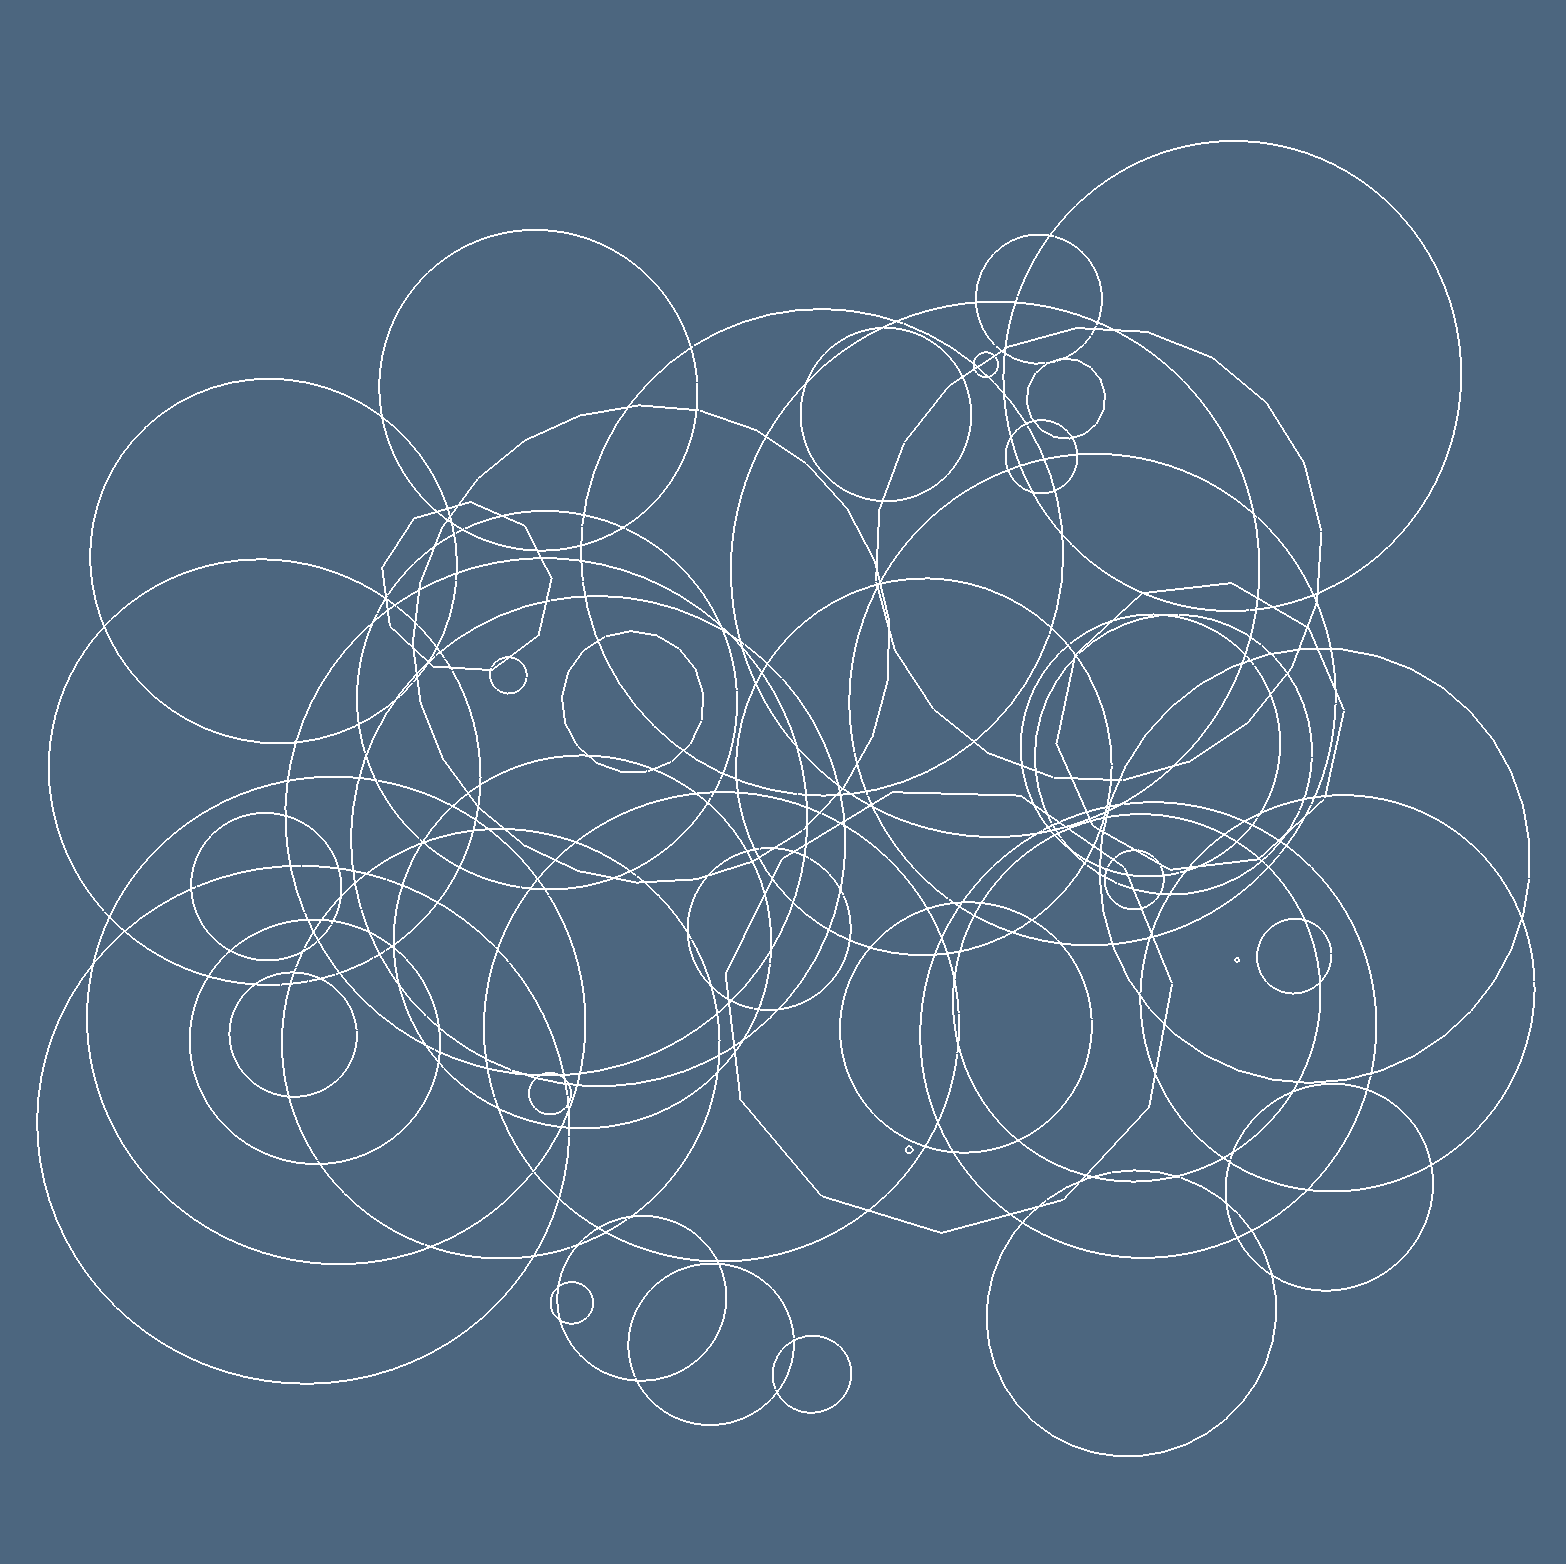
\includegraphics[width=0.5\linewidth]{figs/bubble1.png}%
   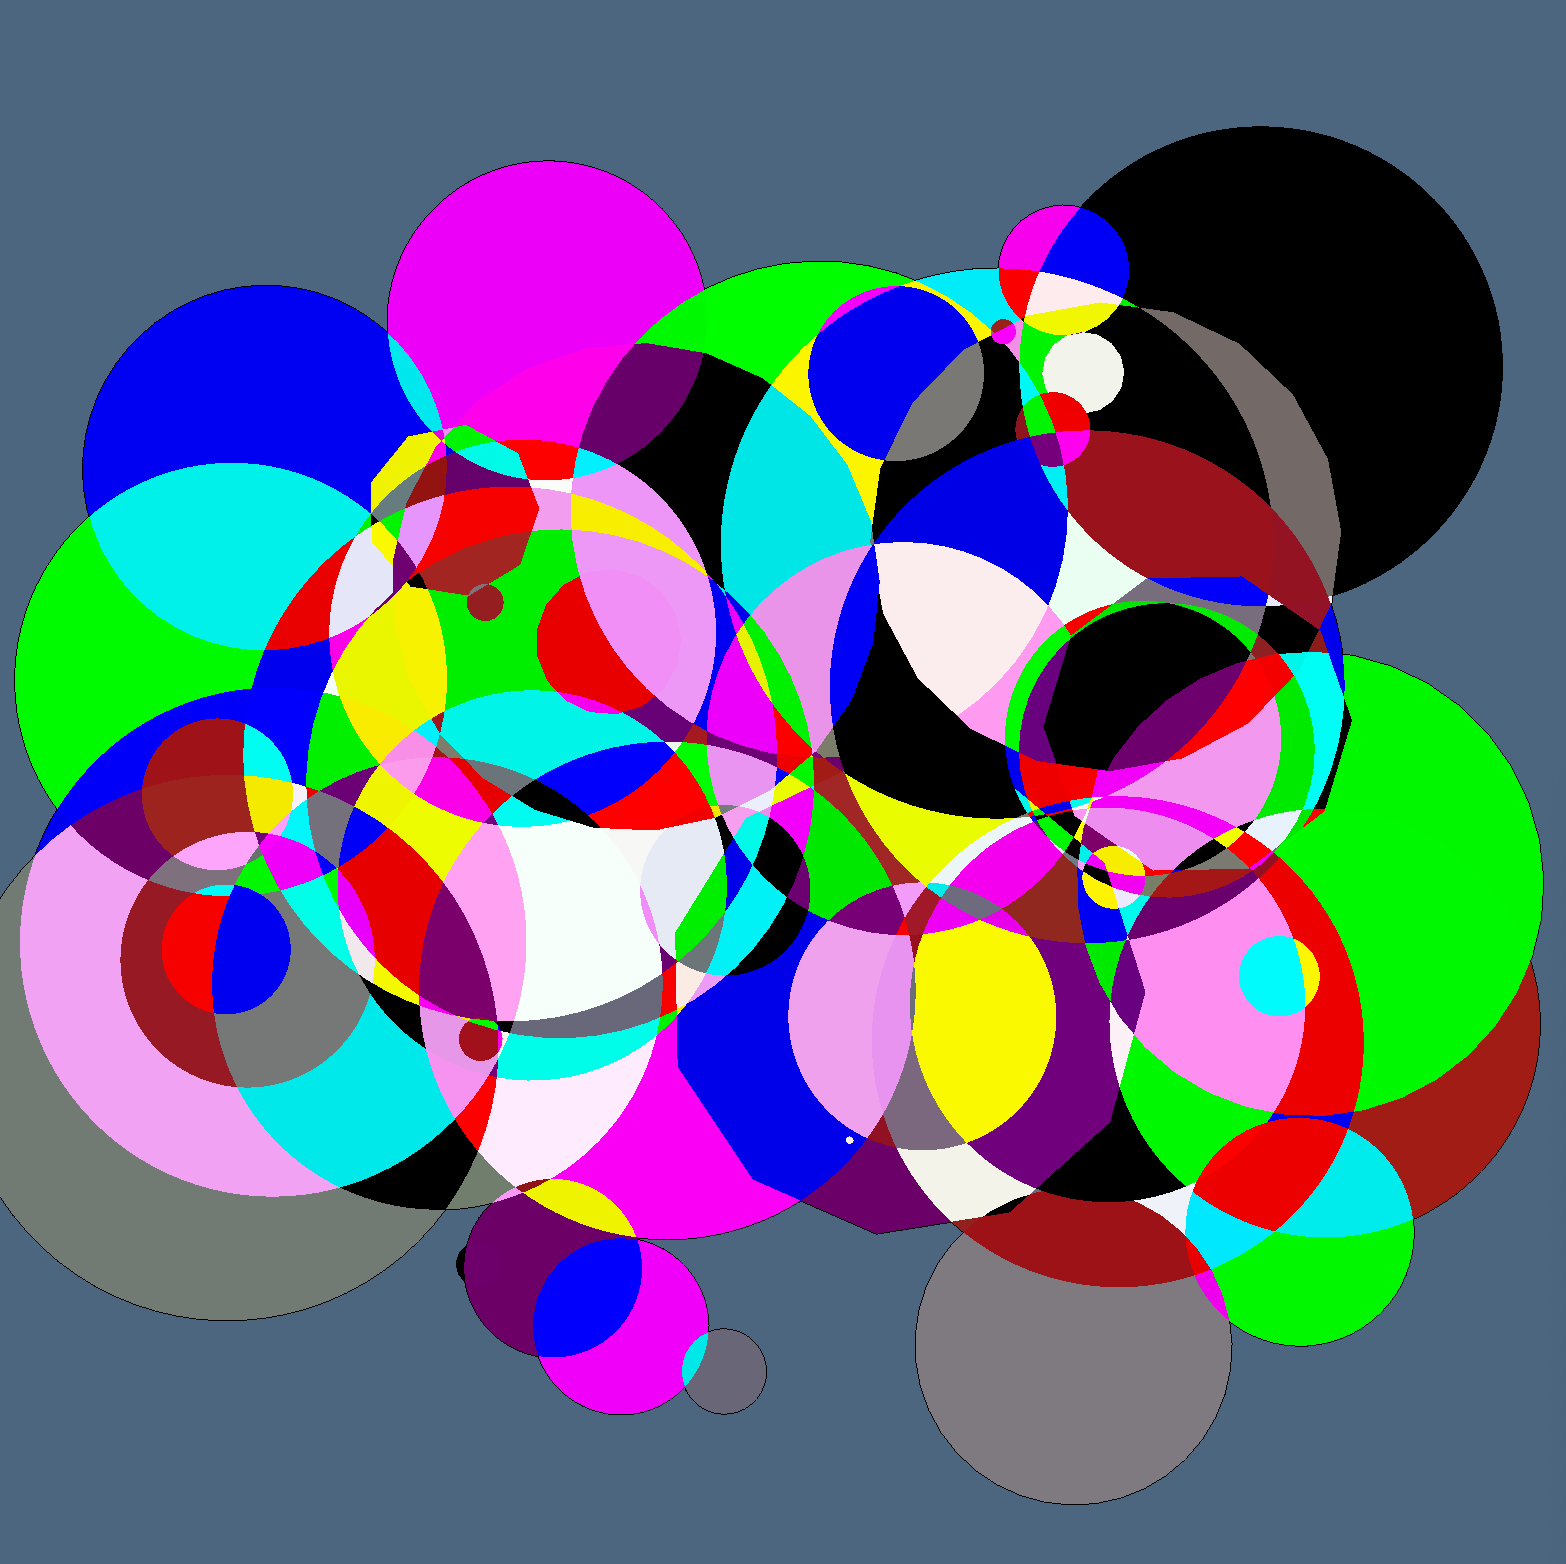
\includegraphics[width=0.5\linewidth]{figs/bubble2.png}%
   
   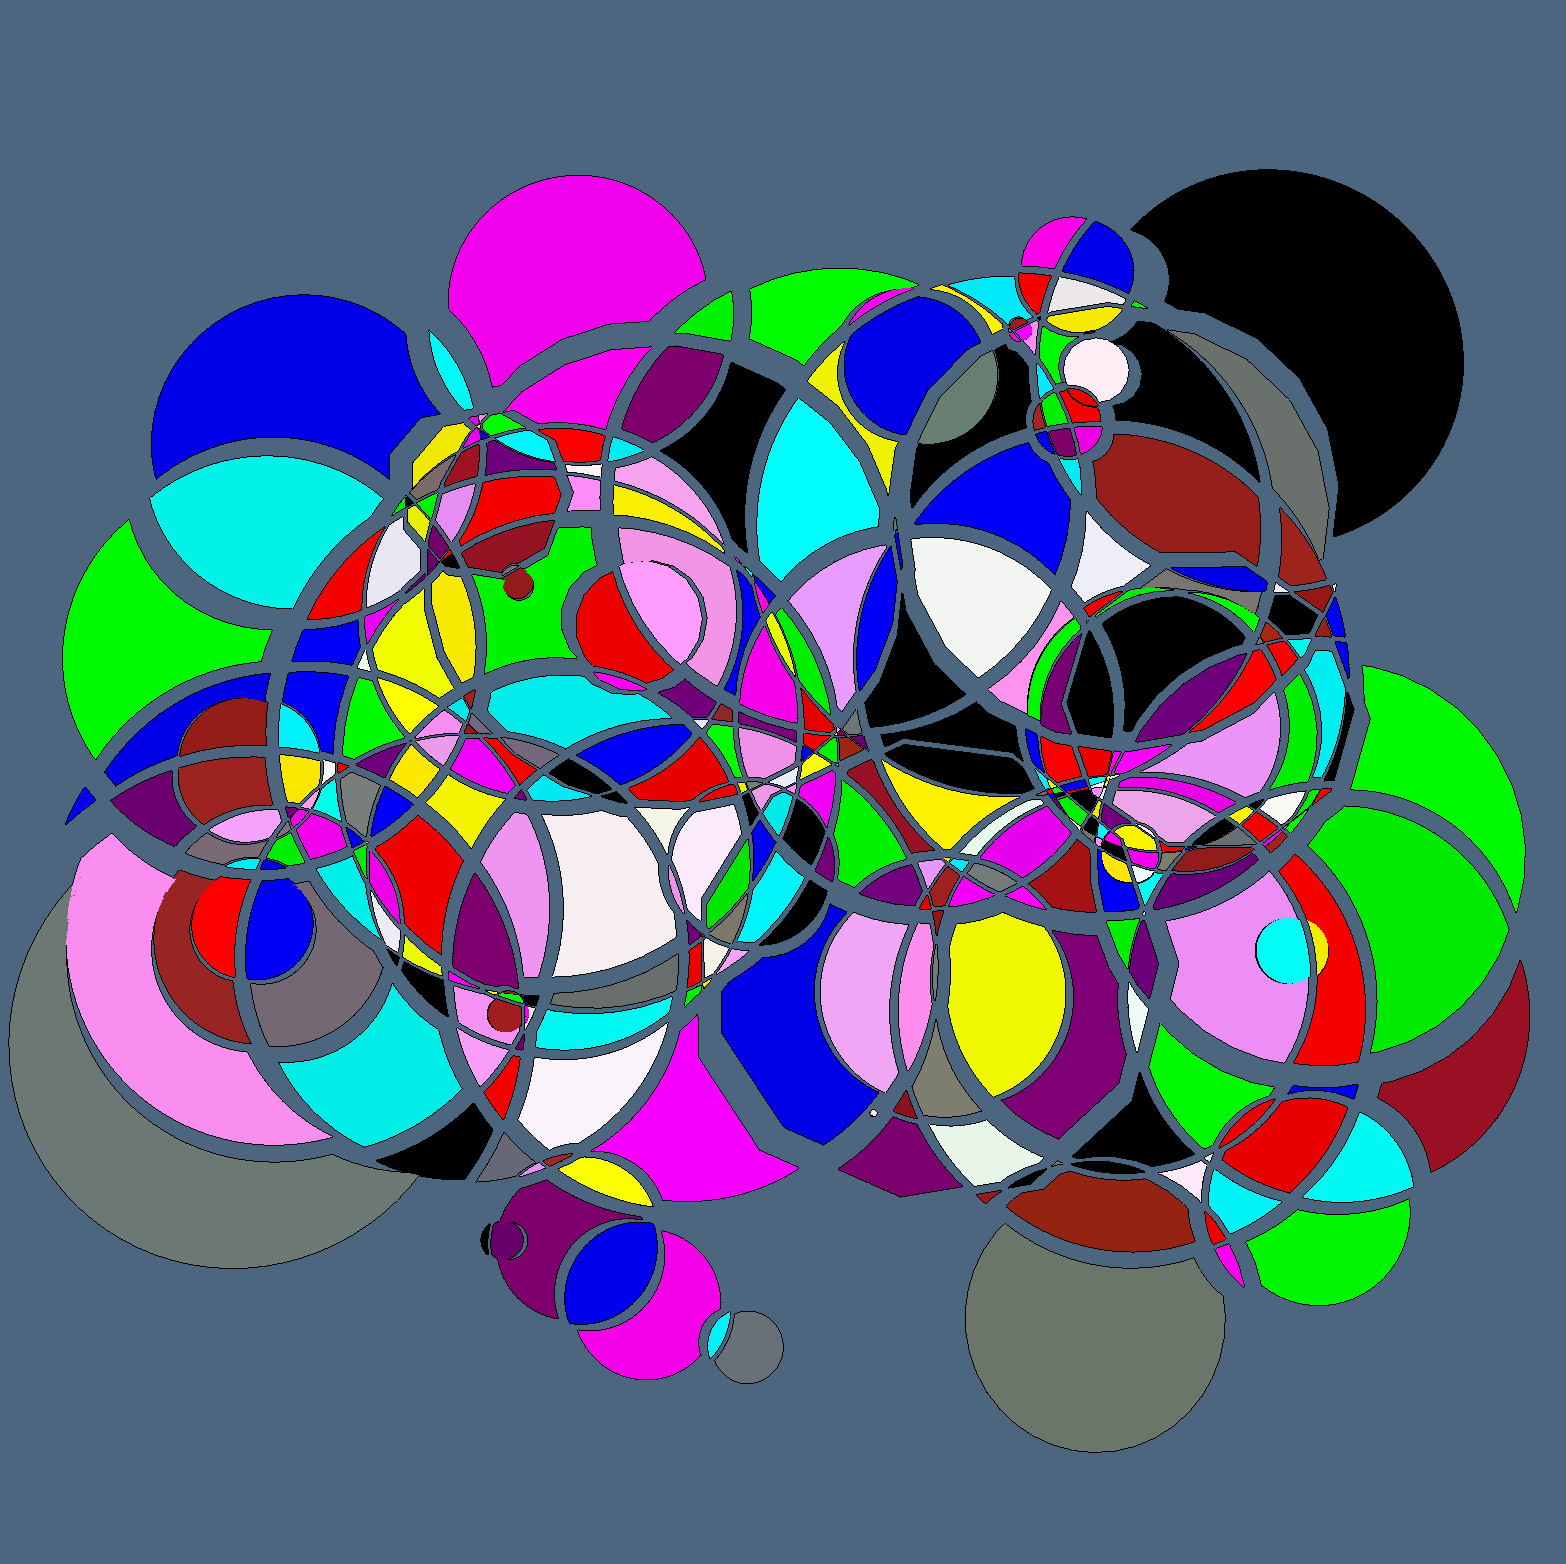
\includegraphics[width=0.5\linewidth]{figs/bubble3.png}%
   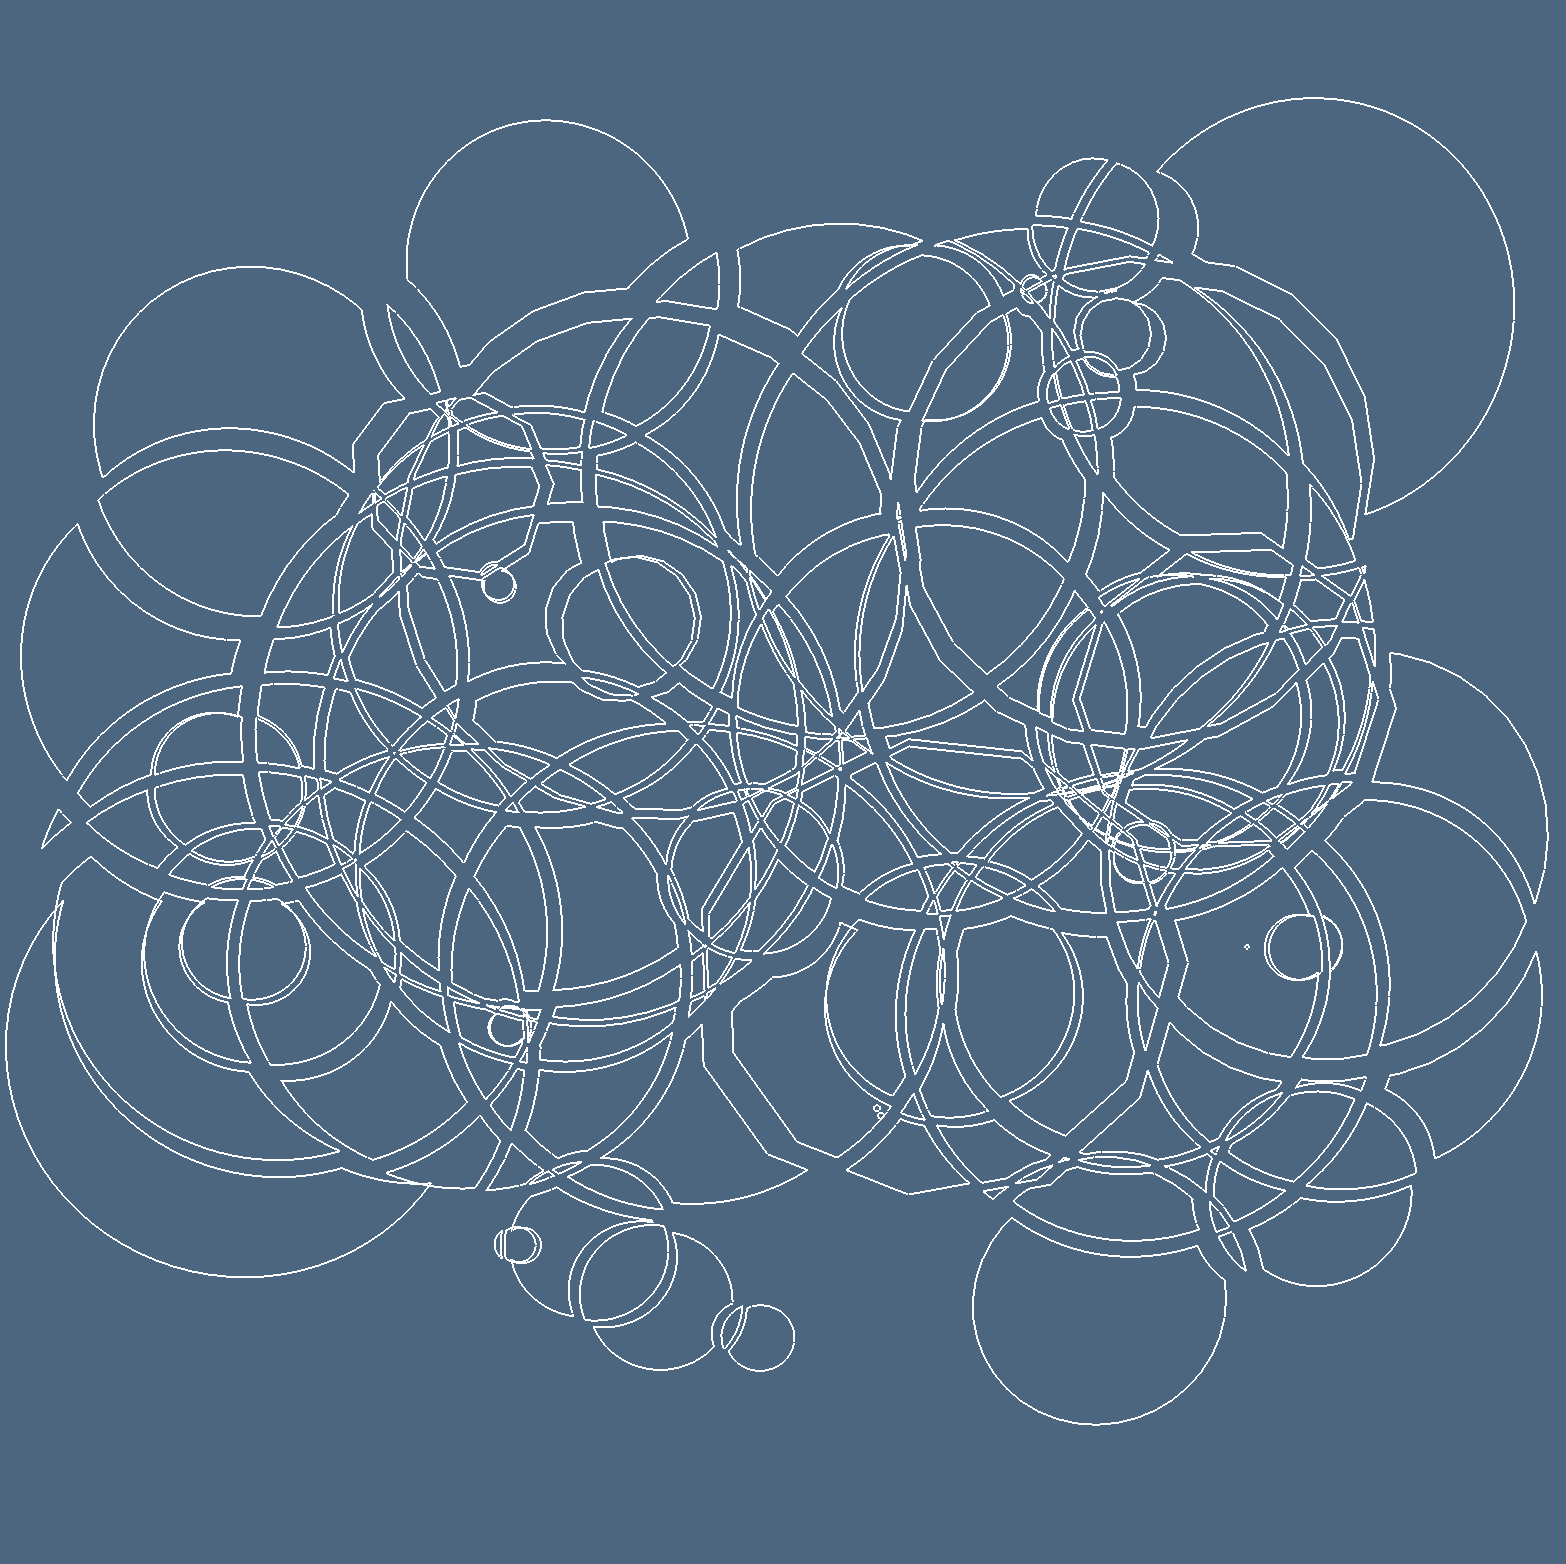
\includegraphics[width=0.5\linewidth]{figs/bubble4.png}%
   \caption{Four views of the 2D arrangement generated by circles and regular polygons:
   (a) the input random polylines; (b) 2-space partition generated by the input; 
   (c) exploded view of the output arrangement; (d) exploded view of boundary 1-cycles of 
   unit 2-chains of the 2-space arrangement.}
   \label{fig:example}
\end{figure}


\begin{figure}[htb] %  figure placement: here, top, bottom, or page
   \centering
   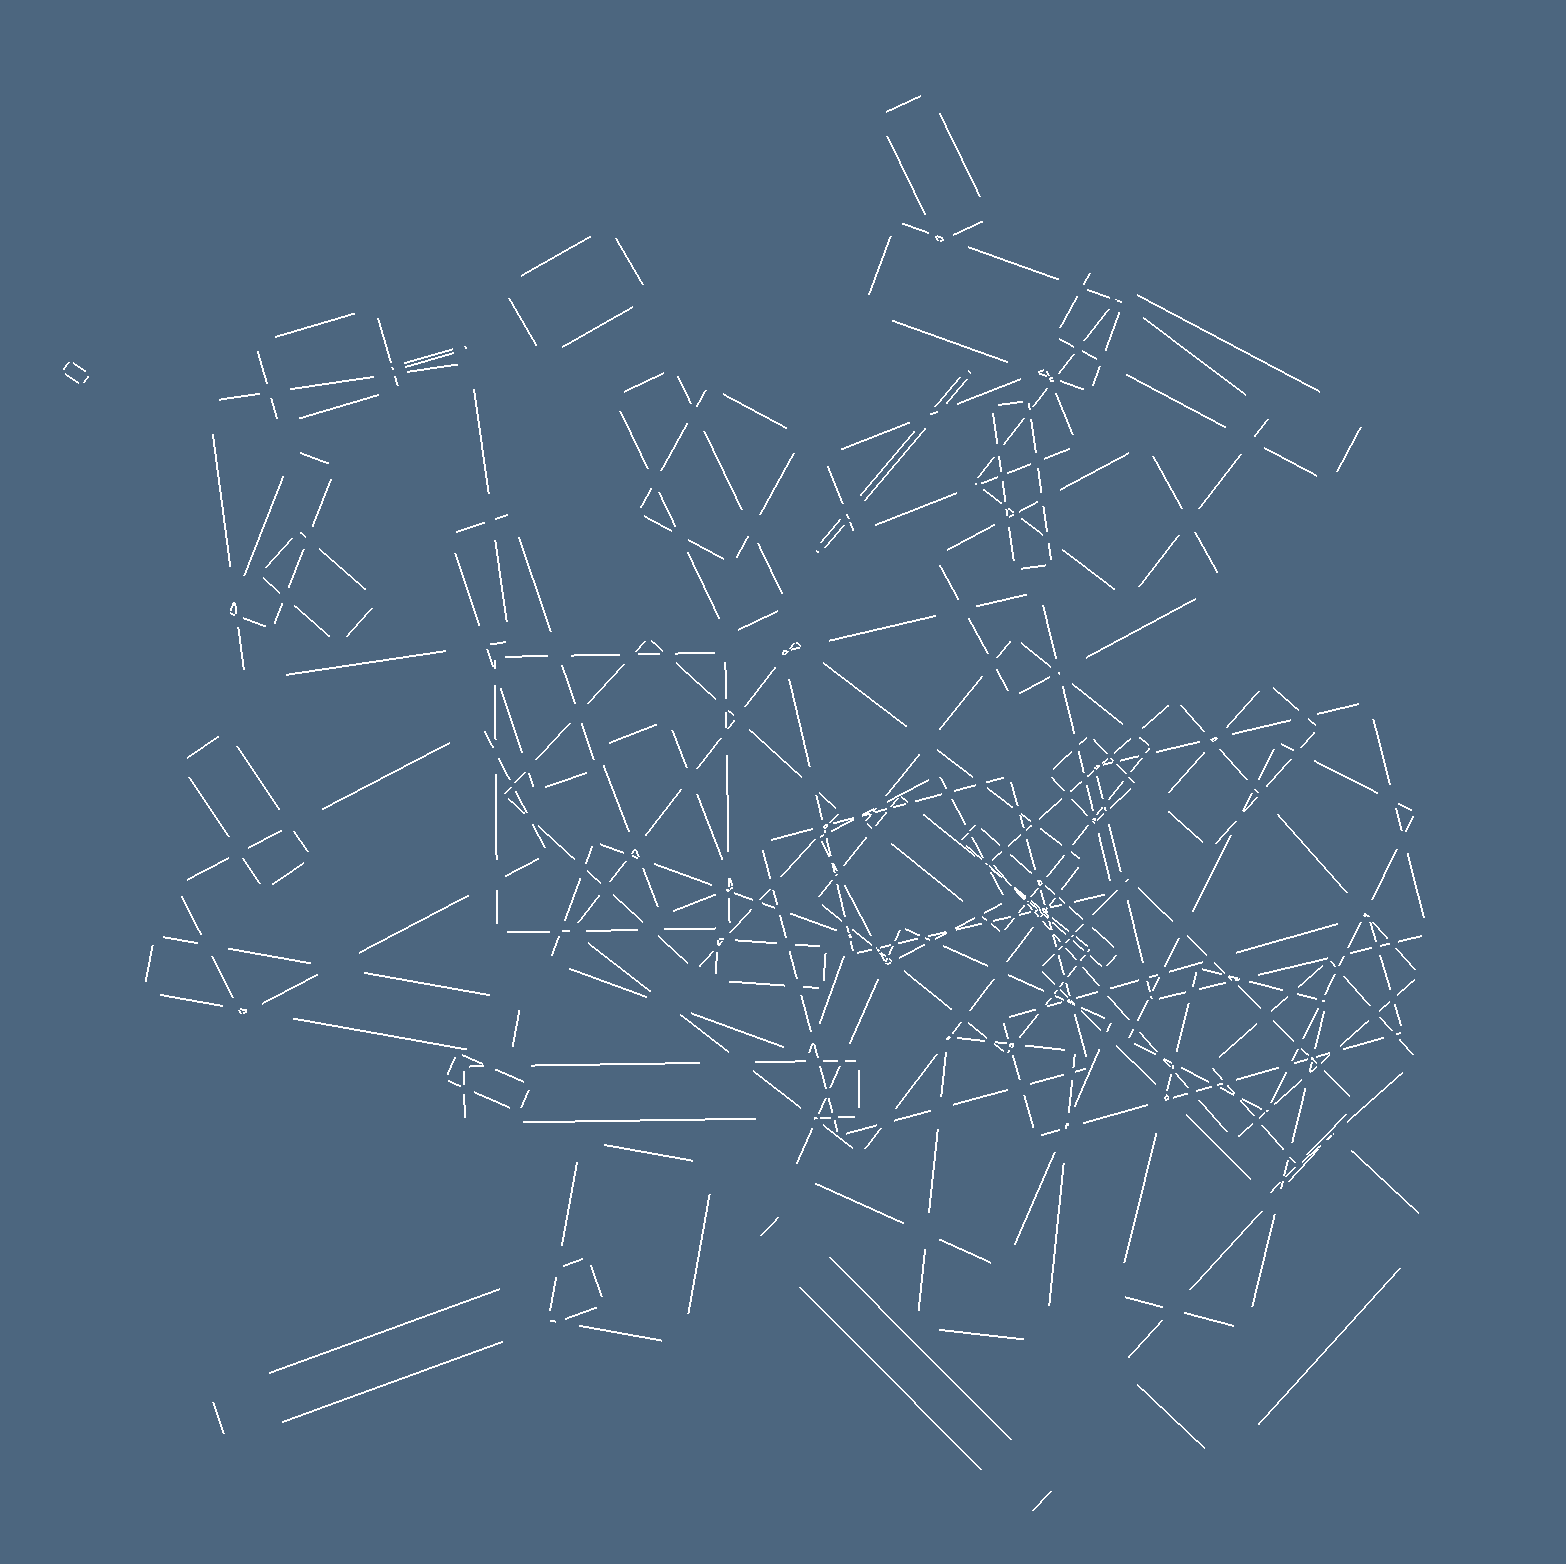
\includegraphics[width=0.5\linewidth]{figs/squares1.png}%
   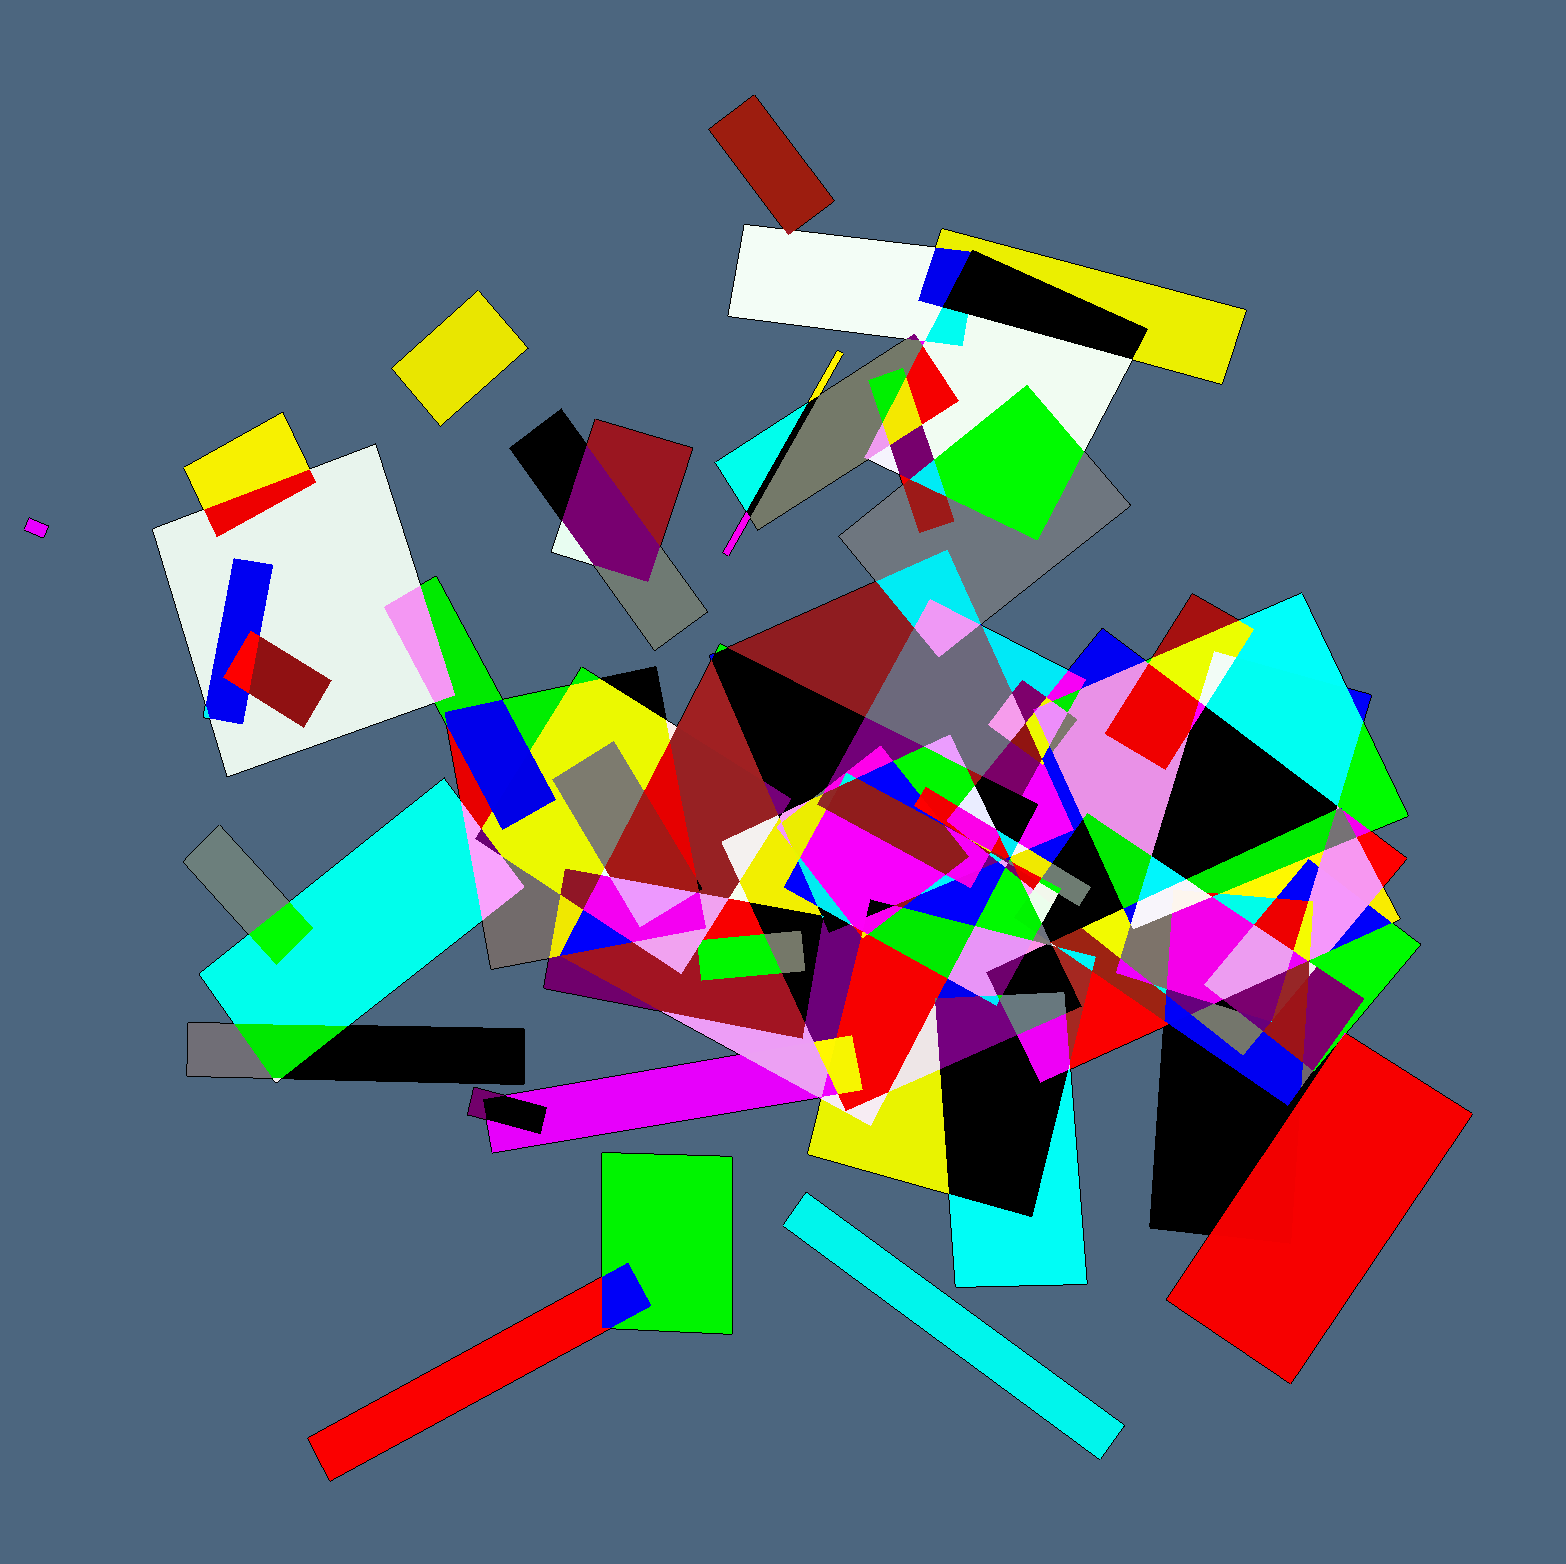
\includegraphics[width=0.5\linewidth]{figs/squares2.png}
   
   \caption{Two views of the 2D arrangement generated by random rectangles:
   (a) exploded view of fragmented 1-chain generated by the input boundaries of rectangles; 
   (b) the 2-space arrangement generated by the input.}
   \label{fig:example}
\end{figure}



\subsection{Boolean 3D workflow}\label{sec:boolean}\footnote{You may enjoy trying \texttt{Lar.cuboidGrid([2,2,2],true)}}
%--------------------------------------------------------------------------------
First define \texttt{cube} as a single element of a grid of cubes:

{\footnotesize\begin{verbatim}
using LinearAlgebraicRepresentation, ViewerGL, SparseArrays
Lar = LinearAlgebraicRepresentation; GL = ViewerGL
V,(VV,EV,FV,CV) = Lar.cuboidGrid([1,1,1],true)
cube = V,FV,EV
\end{verbatim}}

Then position three instances of cubes in $\E^3$ within a hierarchical scene graph, using the \texttt{Struct} function:

{\footnotesize\begin{verbatim}
threecubes = Lar.Struct([ cube,
	Lar.t(.3,.4,.25),Lar.r(pi/5,0,0),Lar.r(0,0,pi/12),cube,
	Lar.t(-.2,.4,-.2),Lar.r(0,pi/5,0),Lar.r(0,pi/12,0),cube ]);
\end{verbatim}}

Convert \texttt{threecubes} to single (self-intersecting) model \texttt{V,FV,EV}, and visualize the collection \texttt{FV} of faces (2-cells). It is not a cellular complex, since cells intersect out of boundaries. See Figure~\ref{fig:threecubes}a:

{\footnotesize\begin{verbatim}
V,FV,EV = Lar.struct2lar(threecubes)
GL.VIEW([ GL.GLGrid(V,FV), GL.GLFrame ])
\end{verbatim}}

Next, prepare the input data types for computing the 3-space arrangement. 
We have to yet better define the  IDE. \texttt{Lar.Cells} and \texttt{Lar.ChainOp} are array or sparse matrix of $p$-cells, respectively.

{\footnotesize\begin{verbatim}
cop_EV = Lar.coboundary_0(EV::Lar.Cells);
cop_EW = convert(Lar.ChainOp, cop_EV);
cop_FE = Lar.coboundary_1(V,FV::Lar.Cells,EV::Lar.Cells);
W = convert(Lar.Points, V');
\end{verbatim}}

$[\delta_2],\;[\delta_1],\;[\delta_0]=\texttt{ChainOp[copCF}, \texttt{copFE}, \texttt{copEV]}$, \emph{Chain Complex} embedded in $\E^3$ by  $3\times n$ vertex matrix \texttt{V}, is finally generated:

{\footnotesize\begin{verbatim}
V, copEV, copFE, copCF = 
	Lar.Arrangement.spatial_arrangement(W, cop_EW, cop_FE)
\end{verbatim}}

The 8 rows of the $\delta_2: C_2\to C_3$ matrix (below) or the 8 columns of $[\partial_3]=[\delta_2]^t$, $\partial_3: C_3\to C_2$, generate the eight
3-cells of Figure~\ref{fig:threecubes}d.

{\footnotesize\begin{verbatim}
@show Matrix(copCF);
\end{verbatim}}\vspace{-2mm}
{\tiny\begin{verbatim}
Int8[
-1 0 1 0 0 0 1 0 -1 0 -1 0 0 0 -1 1 0 1 0 0 -1 1 0 1 -1 0 0 0 -1 -1 0 1 0 0 -1 0 1 0 0 0 1 -1 0 -1 0 0 1;
 0 -1 0 0 0 1 0 0 0 -1 0 0 0 0 0 0 0 0 0 0 0 0 0 0 0 -1 0 -1 0 0 0 0 0 0 1 0 -1 0 0 0 -1 1 0 1 0 0 -1;
 0 0 0 -1 0 0 0 -1 0 0 0 1 1 0 0 0 -1 0 0 1 0 0 -1 0 0 0 1 0 0 0 0 0 0 -1 0 0 0 0 1 0 0 0 0 0 1 0 0;
 0 0 0 0 -1 0 0 0 0 0 0 0 0 1 0 0 0 0 -1 0 0 0 0 0 0 0 0 0 0 0 1 0 0 1 0 0 0 0 -1 0 0 0 0 0 -1 0 0;
 1 0 -1 0 0 0 -1 0 1 0 1 0 0 0 1 -1 0 -1 0 -1 0 0 1 0 0 0 -1 0 0 0 0 0 -1 0 0 0 0 1 0 0 0 0 -1 0 0 0 0;
 0 0 0 1 0 0 0 1 0 0 0 -1 -1 0 0 0 1 0 0 0 1 -1 0 -1 1 0 0 0 1 1 0 -1 0 0 0 -1 0 0 0 1 0 0 0 0 0 1 0;
 0 1 0 0 0 -1 0 0 0 1 0 0 0 0 0 0 0 0 0 0 0 0 0 0 0 0 0 0 0 0 -1 0 1 0 0 0 0 -1 0 0 0 0 1 0 0 0 0;
 0 0 0 0 1 0 0 0 0 0 0 0 0 -1 0 0 0 0 1 0 0 0 0 0 0 1 0 1 0 0 0 0 0 0 0 1 0 0 0 -1 0 0 0 0 0 -1 0]
\end{verbatim}}



\begin{figure}[htbp] %  figure placement: here, top, bottom, or page
   \centering
   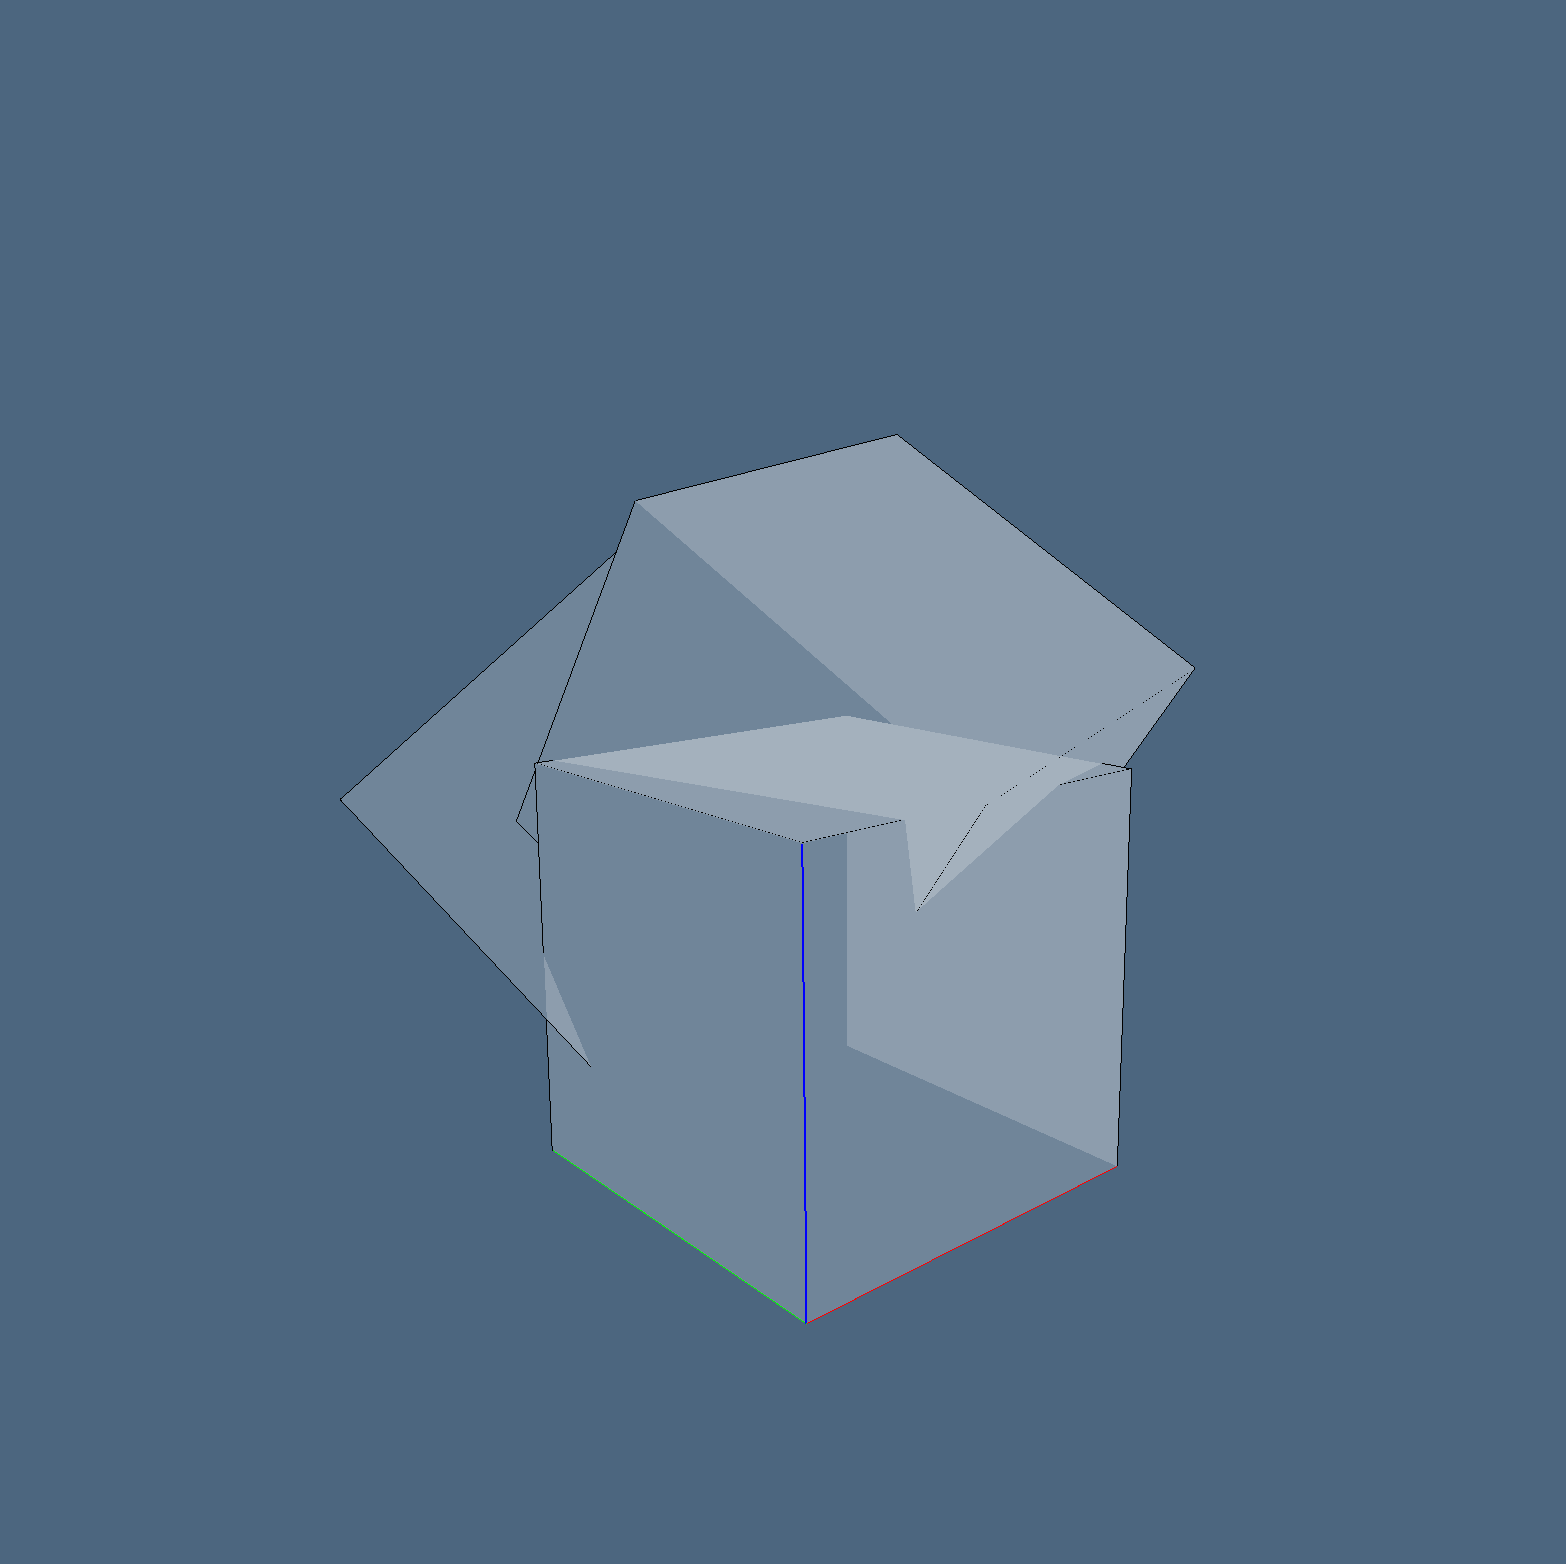
\includegraphics[width=0.5\linewidth]{figs/3cubes1.png}%
   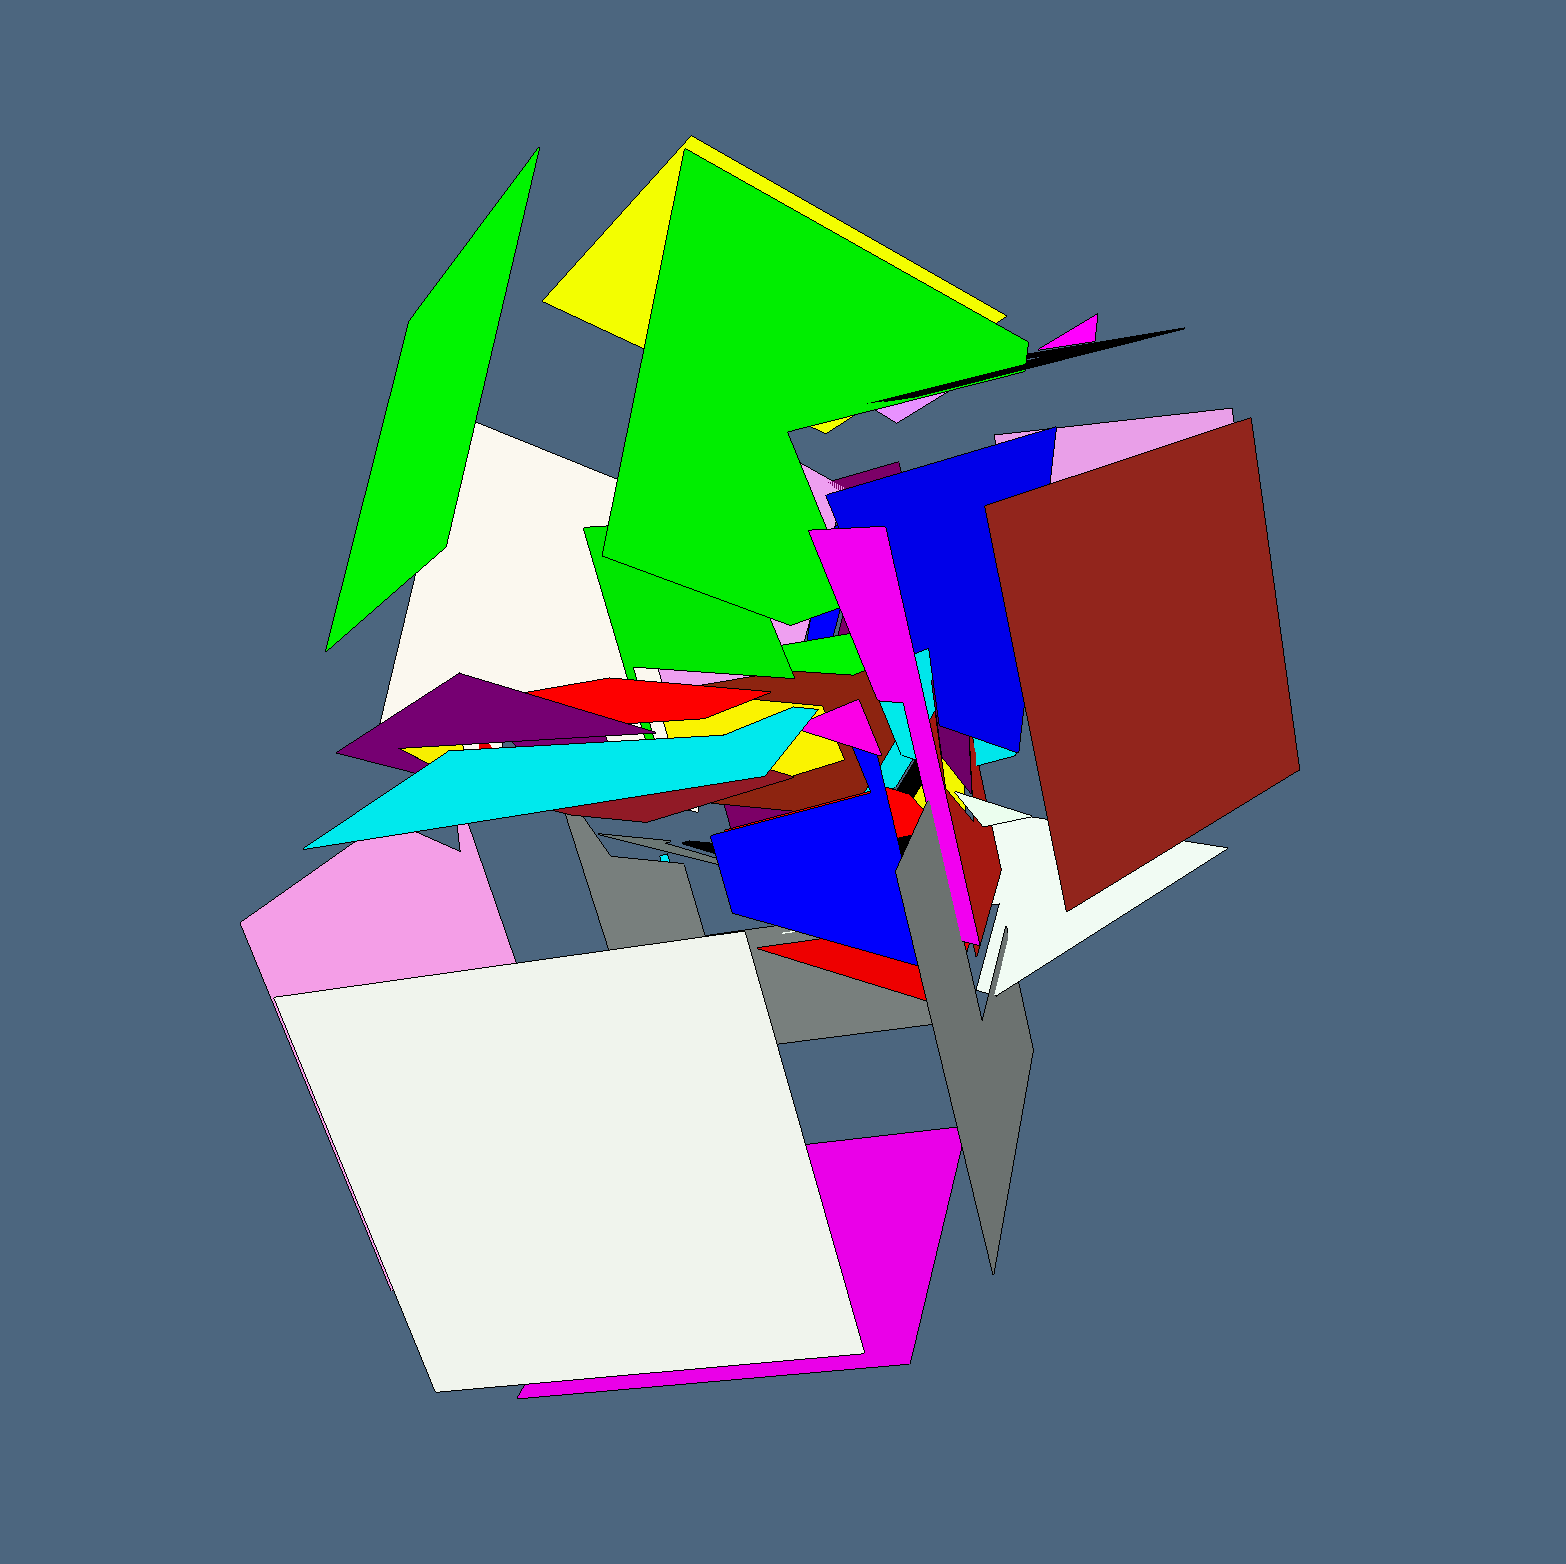
\includegraphics[width=0.5\linewidth]{figs/3cubes2.png}%
   
   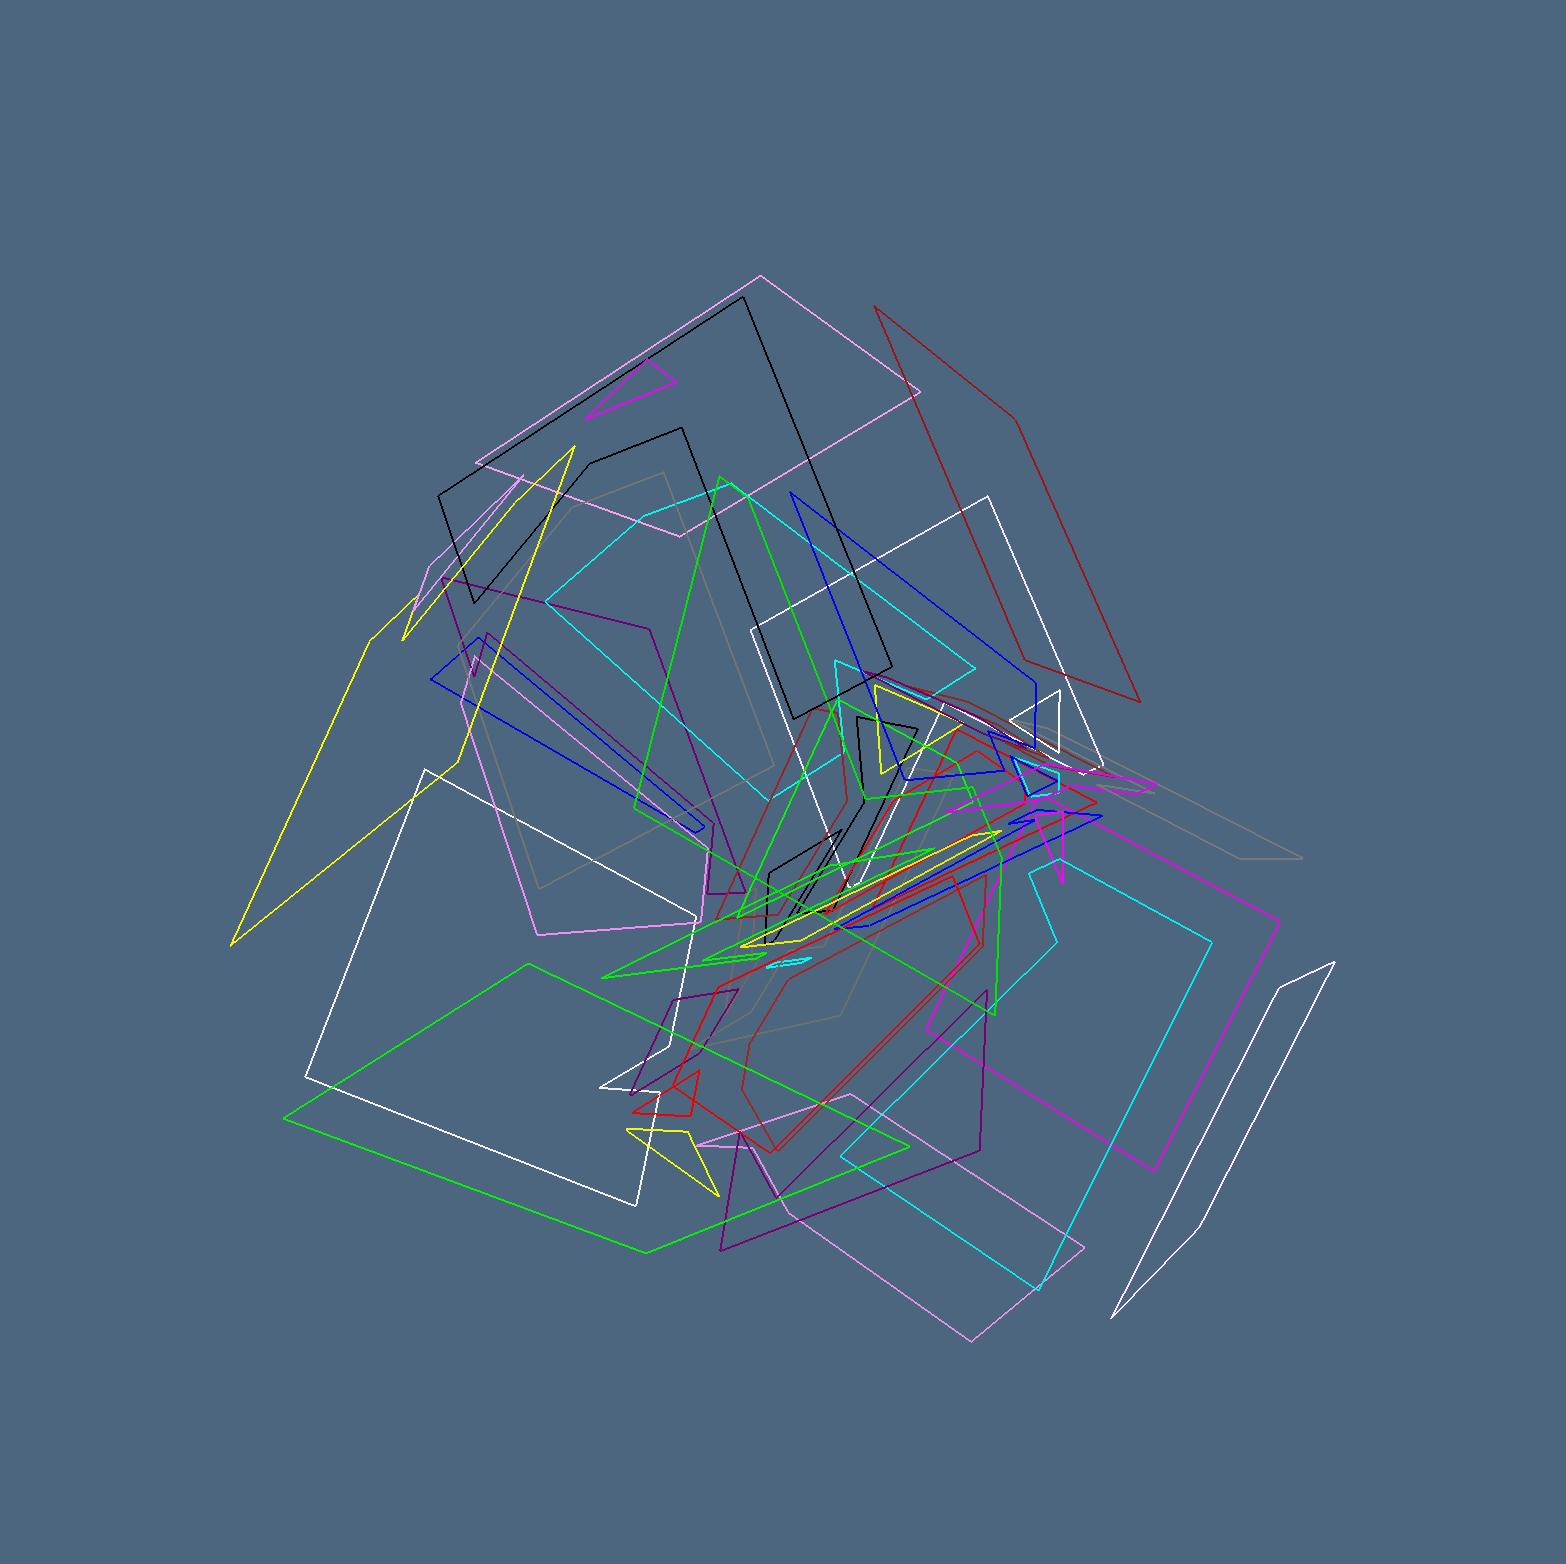
\includegraphics[width=0.5\linewidth]{figs/3cubes3.png}%
   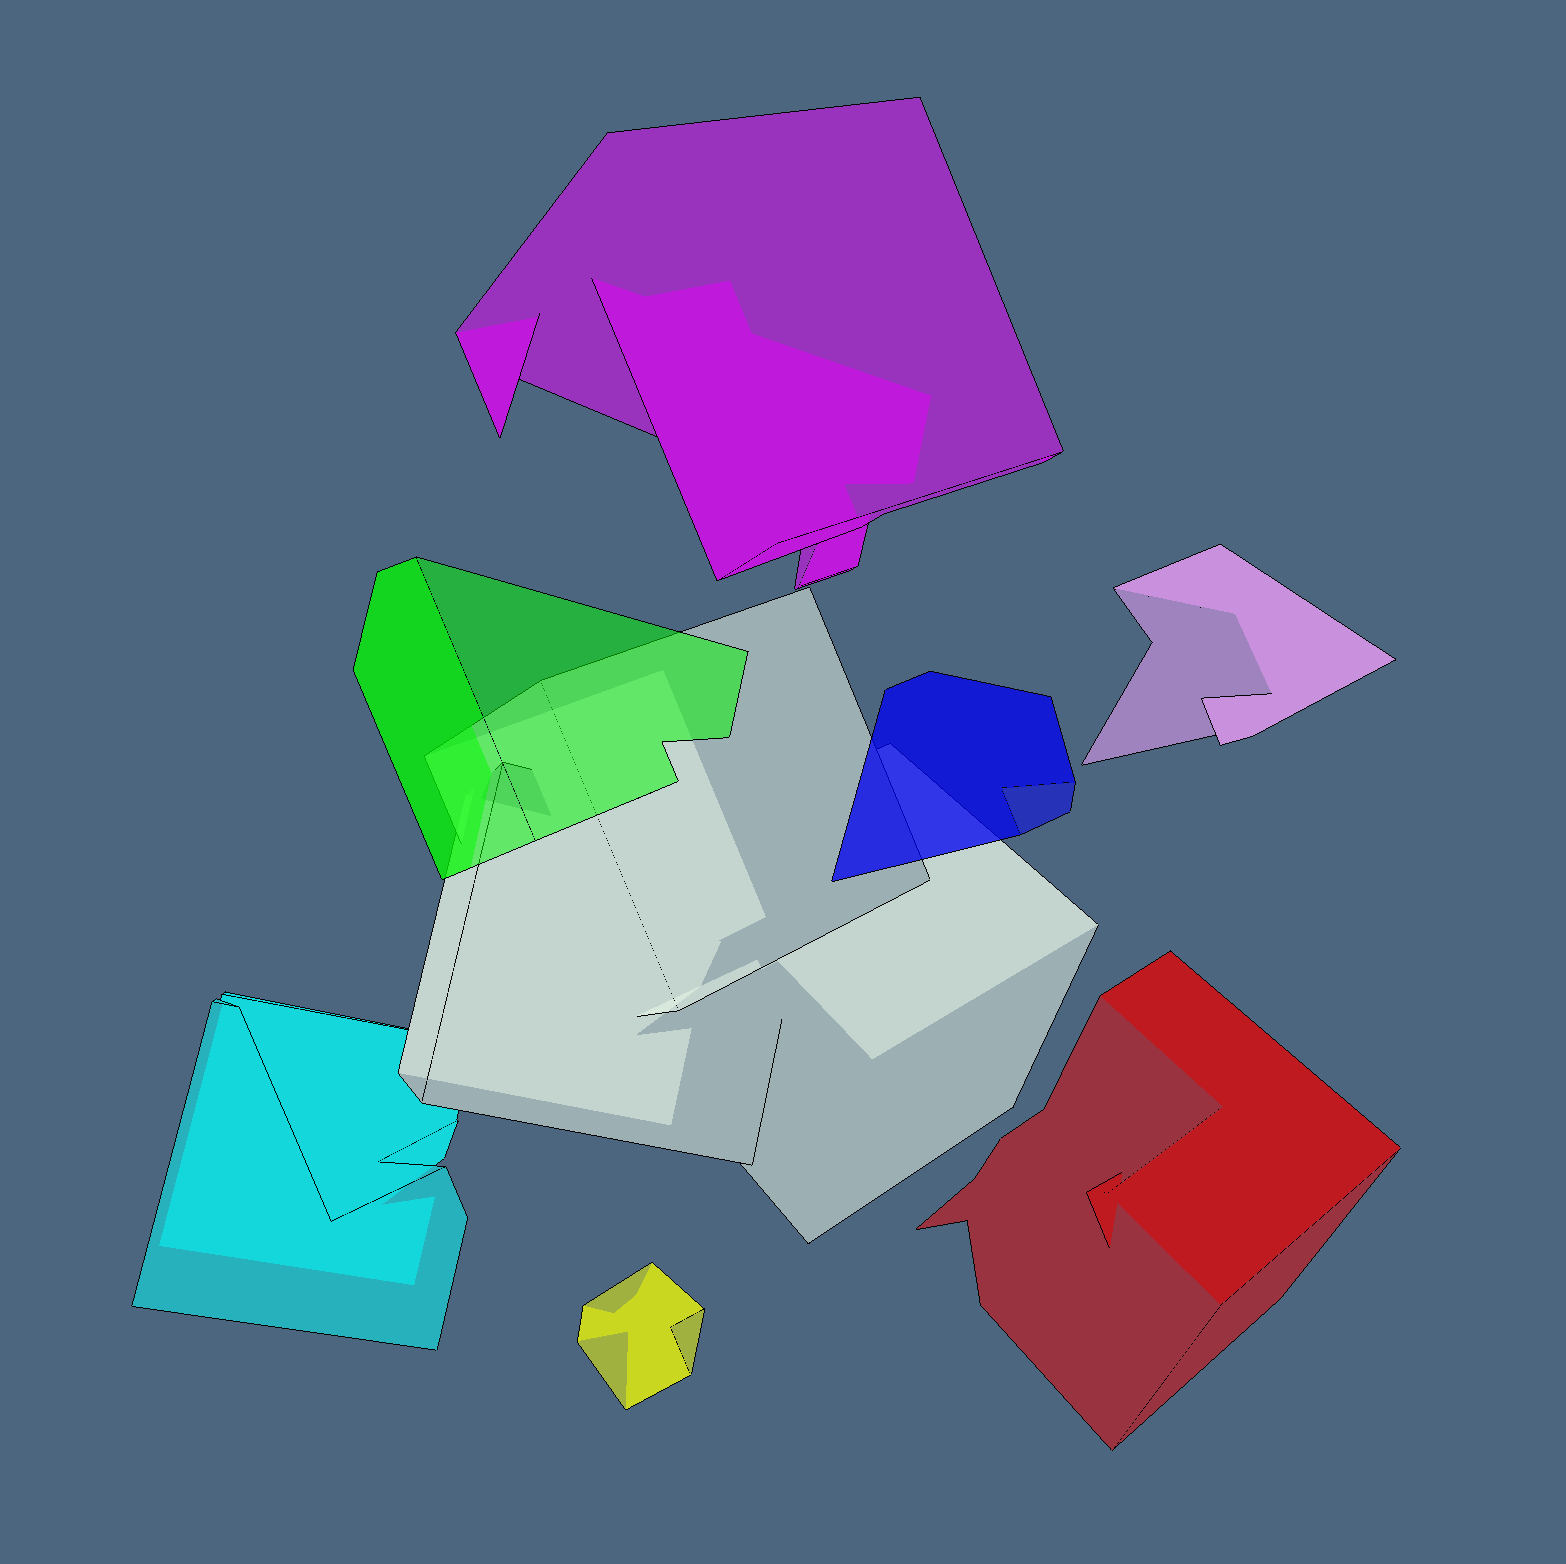
\includegraphics[width=0.5\linewidth]{figs/3cubes4.png}%
  \caption{Images of the 3D arrangement generated by three unit cubes:
   (a) transparent view of the input; (b) exploded 2-skeleton of 3D space partition; 
   (c) exploded view of boundary 1-cycles of 2-cells; (d) exploded view of (transparent) 
   3-chain, which is the basis of 3-space arrangement generated by the input. The white 2-cycle is the 
   boundary of outer space.}
  \label{fig:threecubes}
 \end{figure}

Finally, the \texttt{Lar} model is triangulated, via \texttt{Triangle.jl} package, giving CDT (constrained Delaunay Triangulation), and converted to triangle arrays per 3-cell, per 2-cell, and per  polygon boundary:

{\footnotesize\begin{verbatim}
W = convert(Lar.Points, V')
V,CVs,FVs,EVs = Lar.pols2tria(W, copEV, copFE, copCF)
\end{verbatim}}



{\footnotesize\begin{verbatim}
GL.VIEW(GL.GLExplode(V,FVs,1.5,1.5,1.5,99,1));
GL.VIEW(GL.GLExplode(V,EVs,1.5,1.5,1.5,99,1));
meshes = GL.GLExplode(V,CVs[1:end],8,4,6,99,0.5);
GL.VIEW( push!( meshes, GL.GLFrame) );
\end{verbatim}}


%================================================================================
\section*{Acknowledgements}
%================================================================================
The author is grateful to Antonio DiCarlo and Vadim Shapiro for sharing a lasting curiosity in the exploration of novel geometric territories, and to Giorgio Scorzelli, Francesco Furiani and Giulio Martella for help with the software.

%================================================================================
\section{Conclusion}
%================================================================================
In this paper a very simple and general approach to geometric and topological computing using only Julia's~\cite{bezanson2017julia} sparse arrays was presented. Sparse arrays should fit well with the fast diffusion of hybrid architectures and their advanced applications, using the best-in-class numerical language. The future applications may cover disparate fields of visual calculus, including geomapping, solid and geometric computer-aided design, virtual reality, computer vision, and medical imaging.  
We are just at the beginning of this journey. A lot of work remains, and this author has strong hope to share the enjoyment of discovery with the Julia's community.


\bibliographystyle{juliacon}
\scriptsize
\bibliography{ref}


%% **************GENERATED FILE, DO NOT EDIT**************

\bibliographystyle{juliacon}
\bibliography{ref.bib}


\end{document}

% Inspired by the International Journal of Computer Applications template
